\documentclass[11pt,letterpaper,onecolumn]{article}

\usepackage{hexopaper}
\usepackage{hexfig}

\title{Certified Defender Move Restriction in Hexo Threat Search}
\author{Cmiller132}
\date{July 2026}

\begin{document}

\maketitle

\begin{abstract}
Threat-space search in Hexo has large defender branching because every legal
reply must ordinarily be considered.  We develop a horizon-parameterized
certificate that restricts defender replies while preserving a proved
attacker win over the full legal move set.  Companion results establish the
impossibility of a global pairing defense, a potential-function layer for
blocking certificates, local domination patterns, and mechanized validation
of the finite claims and move-set closure.
\end{abstract}

\section{Introduction}
\label{sec:introduction}

A df-pn threat-space solver must, at a defender AND node, in principle
consider every legal reply.  In Hexo this means every empty cell within hex
distance 8 of any existing stone, often hundreds of cells.  Enumerating these
replies dominates the cost of the search.

The restriction studied here is \emph{certified}: every omitted defender
reply has a verifier-checkable proof of sound dismissal.  Search trimming may
cause the solver to miss an attacker win, so it can reduce completeness.  It
cannot cause a false attacker win to pass verification.  This separation
between completeness and soundness holds regardless of the heuristic used to
generate the searched replies.

The restriction must depend on a finite horizon.  No fixed static set is
sufficient for every future continuation on the unbounded board.  A
certificate instead states its own placement horizon and carries the zone
obligations needed up to that horizon.

The paper first gives the formal game model in \cref{sec:game} and the
locality lemmas in \cref{sec:geometry}.  It then defines zone-carrying
certificates in \cref{sec:certificates} and proves horizon-parameterized
dismissal soundness in \cref{sec:main-theorem}.  The computable constructions
of \cref{sec:computable-zones} include a measured generator mean of 147 cells,
compared with 302 legal cells.  The remaining layers establish the
impossibility of a global pairing defense in \cref{sec:no-pairing}, develop
potential-function certificates in \cref{sec:potential}, give local
domination patterns in \cref{sec:domination}, and report mechanized validation
in \cref{sec:validation}.

Threat-space search and proof-number methods provide the search setting for
these certificates \cite{allis-1994,nagai-2002}.  Pairing strategies and the
potential method are standard tools for positional games
\cite{erdos-selfridge-1973,beck-2008}.

The full internal proof documents, review history, and validation scripts are
available in the repository \cite{hexobot-companions}.

\section{The game and formal model}
\label{sec:game}

\subsection{Informal rules}

Hexo is a two-player placement game on an unbounded hexagonal grid.  The
opening player places one stone at the origin.  Thereafter the players
alternate turns of two placements.  Stones are permanent.  A placement is
legal on any empty cell within hex distance 8 of a stone of either player.
The first player to occupy six consecutive cells on one of the three grid
axes wins.  A win is checked after each placement, so a win on the first
placement ends the game before the second placement of that turn.

We use attacker and defender as fixed roles, denoted by $\A$ and $\D$.  A
ply is one placement, while a normal turn contains two plies.  Everything
below concerns positions after the Opening placement (the origin is occupied;
budgets follow the turn structure of \cref{def:D4}).

\subsection{Formal model}

The first definition fixes the infinite board and the metric used by both
the line geometry and the legality rule.

\begin{definition}[Board, cells, and distance]
\label{def:D1}
The cells are the integer axial lattice $\Cells\ni x=(q,r)$.  For
$x=(q,r)$ and $y=(q',r')$, set
\[
  \dist(x,y)=\max\bigl\{|q-q'|,\ |r-r'|,
                  |(q-q')+(r-r')|\bigr\}.
\]
\end{definition}

The winning patterns are finite segments along the three line directions of
the axial lattice.

\begin{definition}[Axes and windows]
\label{def:D2}
The axis vectors are
\[
  \mathfrak a\in\{(1,0),(0,1),(1,-1)\}.
\]
A \emph{window} is a set
\[
  W=\{s+i\mathfrak a:0\le i\le5\}
\]
for a start cell $s$ and an axis vector $\mathfrak a$.  Every window has
exactly six cells, and every cell lies in exactly 18 windows, from three axes
and six possible offsets on each axis.
\end{definition}

The next fact records the metric consequence of belonging to one window.

\begin{fact}[Window collinearity]
\label{fact:F1}
Two distinct cells of a window differ by a nonzero multiple of the window's
axis vector.  Thus any two cells contained in a common window are collinear
along that axis and have distance at most $5$.
\end{fact}

Figure~\ref{fig:coordinates} shows the coordinate convention and one distance
calculation.

\begin{figure}[tbp]
  \centering
  \begin{tikzpicture}[scale=.88]
    \HexBoardRange{0}{0}{2}
    \foreach \q/\r/\shade in {0/0/22,1/0/10,2/-1/22}{
      \path[fill=black!\shade,draw=none] \HexAt{\q}{\r}
        ++(30:.94) \foreach \angle in {150,210,270,330,30}
        {-- ++(\angle:.94)} -- cycle;
    }
    \node[font=\scriptsize] at \HexAt{-1}{0} {$(-1,0)$};
    \node[font=\scriptsize] at \HexAt{0}{0} {$(0,0)$};
    \node[font=\scriptsize] at \HexAt{1}{0} {$(1,0)$};
    \node[font=\scriptsize] at \HexAt{2}{0} {$(2,0)$};
    \node[font=\scriptsize] at \HexAt{0}{1} {$(0,1)$};
    \node[font=\scriptsize] at \HexAt{2}{-1} {$(2,-1)$};
  \end{tikzpicture}
  \caption{Pointy-top axial coordinates.  The shaded cells show a shortest
  path from $(0,0)$ to $(2,-1)$, and
  $d=\max(|2|,|-1|,|1|)=2$.}
  \label{fig:coordinates}
\end{figure}

A position records the finite board state and the exact placement remaining
in the current turn.

\begin{definition}[Positions]
\label{def:D3}
A position is $P=(\sigma,m,b)$, where $\sigma$ is a finite partial map
$\Cells\rightharpoonup\{\A,\D\}$, the mover is
$m\in\{\A,\D\}$, and $b\in\{1,2\}$ is the mover's number of remaining
placements in the current turn.  Stones are permanent, and
$\Stones(P)=\operatorname{dom}\sigma$.  For $X\in\{\A,\D\}$, let $\bar X$
denote the other player.  For such an $X$ and a window
$W$, define
\[
  \cnt_X(W,P)=|\{c\in W:\sigma(c)=X\}|.
\]
When the position is clear from context, we suppress it and write
$\cnt_X(W)$.
\end{definition}

Legality is local to the existing stones, while a transition must also
account for immediate termination and the two-placement turn structure.

\begin{definition}[Legality and transitions]
\label{def:D4}
A cell $c$ is \emph{legal} in $P$ if and only if
\[
  c\notin\operatorname{dom}\sigma
  \quad\text{and}\quad
  \exists s\in\operatorname{dom}\sigma:\dist(c,s)\le8.
\]
Write $\Legal(P)$ for the set of cells legal in $P$.
The mover places on a legal cell $c$, producing
$\sigma'=\sigma\cup\{c\mapsto m\}$.  If some window $W$ then satisfies
$\cnt_m(W)=6$, the game terminates immediately and $m$ wins.  Wins are
therefore checked after each placement and may occur on the first placement
of a two-placement turn.  If there is no win, the next position is
$ (\sigma',m,1)$ when $b=2$, and $(\sigma',\bar m,2)$ when $b=1$.
\end{definition}

Window states distinguish usable winning lines, blocked lines, and lines that
can be completed within one normal turn.

\begin{definition}[Window states]
\label{def:D5}
A window $W$ is \emph{alive for $X$} if
$\cnt_{\bar X}(W)=0$.  An all-empty window is alive for both players.  It is
\emph{dead} if $\cnt_\A(W)\ge1$ and $\cnt_\D(W)\ge1$.  It is an
\emph{$X$-threat} if it is alive for $X$ and $\cnt_X(W)\ge4$.
\end{definition}

The three panels in \cref{fig:window-states} give the basic mask patterns used
by this terminology.

\begin{figure}[tbp]
  \centering
  \begin{subfigure}[t]{.30\textwidth}
    \centering
    \begin{tikzpicture}[scale=.38]
      \HexPatch{0/0,1/0,2/0,3/0,4/0,5/0}
      \HexWindow[window one]{0}{0}{1}{0}
      \HexAttacker{1}{0}\HexAttacker{4}{0}
    \end{tikzpicture}
    \caption{Alive for $\A$.}
  \end{subfigure}\hfill
  \begin{subfigure}[t]{.30\textwidth}
    \centering
    \begin{tikzpicture}[scale=.38]
      \HexPatch{0/0,1/0,2/0,3/0,4/0,5/0}
      \HexAttacker{1}{0}\HexDefender{4}{0}
    \end{tikzpicture}
    \caption{Dead.}
  \end{subfigure}\hfill
  \begin{subfigure}[t]{.30\textwidth}
    \centering
    \begin{tikzpicture}[scale=.38]
      \HexPatch{0/0,1/0,2/0,3/0,4/0,5/0}
      \HexWindow[window two]{0}{0}{1}{0}
      \HexAttacker{0}{0}\HexAttacker{1}{0}
      \HexAttacker{3}{0}\HexAttacker{4}{0}
    \end{tikzpicture}
    \caption{An $\A$-threat with count $4$.}
  \end{subfigure}
  \caption{Alive, dead, and threat window states.  Filled disks are attacker
  stones and open disks are defender stones.}
  \label{fig:window-states}
\end{figure}

The implemented one-ply analysis tests whether the mover can win in the
remaining placements or whether the opponent's threats exceed the defensive
budget.

\begin{definition}[$\lambda^1$ predicates]
\label{def:D6}
For mover $m$ with budget $b$, $\ownwinnow(P)$ holds if and only if there is
an $m$-alive window $W$ such that
\[
  \cnt_m(W)=5,
  \qquad\text{or}\qquad
  \cnt_m(W)=4\ \text{ and }\ b=2.
\]
The value $\hit(P)$ is the multiset of empty-cell sets of the
$\bar m$-threat windows.  The value $\mhs(P)$ is the minimum number of cells
meeting every set in $\hit(P)$, computed exhaustively for values at most $2$.
The $\lambda^1$ verdict is \textsc{win} when $\ownwinnow(P)$ holds,
\textsc{loss} when it does not hold and $\mhs(P)>b$, and undecided otherwise.
The post-opening soundness of these implemented verdicts is assumed here.
\end{definition}

Absolute placement indices allow later certificates to state an exact win
horizon without treating a two-placement turn as simultaneous.

\begin{definition}[Plies and horizon]
\label{def:D7}
A \emph{ply} is one placement, and ply indices are absolute along a play.  For
a position $P$ with mover $m$, the \emph{defender-placement count before ply
$T$}, written $\DefCount(P,T)$, is the number of plies strictly before $T$ at
which $\D$ places, as determined by $(m,b)$ and alternation.
\end{definition}

The final convention fixes the direction needed when defender replies are
removed from an attacker-win certificate.

\begin{definition}[Dominance direction]
\label{def:D8}
Outcomes are evaluated for the attacker $\A$, with
$\mathrm{WIN}\succ\nonWIN$.  A \emph{sound dismissal} of a defender reply
$c$ at a node $N$ means that, if the certificate proves that $\A$ wins against
all searched replies, then $\A$ also wins against $c$.
\end{definition}

\begin{figure}[tbp]
  \centering
  \begin{tikzpicture}[scale=.46]
    \HexPatch{0/-4,1/-4,-1/-3,0/-3,1/-3,-1/-2,0/-2,1/-2,2/-2,
      -1/-1,0/-1,1/-1,2/-1,3/-1,4/-1,5/-1,
      -2/0,-1/0,0/0,1/0,2/0,3/0,4/0,5/0,
      -2/1,-1/1,0/1,1/1,2/1,3/1,4/1,
      -3/2,-2/2,-1/2,0/2,1/2,
      -4/3,-3/3,-2/3,-1/3,0/3,
      -5/4,-4/4,-3/4,-5/5,-4/5}
    \HexWindow[fill=black!8,draw=none]{-1}{0}{1}{0}
    \HexWindow[fill=black!18,draw=none]{0}{-3}{0}{1}
    \HexWindow[fill=black!30,draw=none]{-4}{4}{1}{-1}
    \HexMark{0}{0}{dot}{}
    \draw[-{Stealth[length=4pt]},line width=.55pt]
      \HexAt{5.75}{0} -- \HexAt{6.30}{0};
    \node[font=\scriptsize,anchor=west] at \HexAt{6.45}{0} {$(1,0)$ axis};
    \draw[-{Stealth[length=4pt]},line width=.55pt]
      \HexAt{0}{3.70} -- \HexAt{0}{4.25};
    \node[font=\scriptsize,anchor=south west] at \HexAt{0}{4.40}
      {$(0,1)$ axis};
    \draw[-{Stealth[length=4pt]},line width=.55pt]
      \HexAt{2.70}{-2.70} -- \HexAt{3.25}{-3.25};
    \node[font=\scriptsize,anchor=north west] at \HexAt{3.40}{-3.40}
      {$(1,-1)$ axis};
  \end{tikzpicture}
  \caption{One six-cell window on each axis through the central cell, shown
  with three fill shades.  Sliding a window so that the cell occupies offsets
  $0$ through $5$ gives $3$ axes $\times$ $6$ offsets $=18$ windows through
  the marked cell.}
  \label{fig:axes-windows}
\end{figure}

\section{Elementary geometry}
\label{sec:geometry}

The first bound relates the number of stones in a window to the maximum gap
from an empty cell to those stones.

\begin{lemma}[Packing bound]
\label{lem:L1}
In a window with $k\ge1$ stones of one colour and no stones of the other,
every empty cell of the window is within distance $6-k$ of a same-window
stone.  The bound is tight.
\end{lemma}

\begin{proof}
Index the cells $0,\ldots,5$ along the window axis.  Let $e$ be empty, and let
$\delta$ be its axis-distance from a nearest in-window stone.  The $\delta$
cells from $e$ toward that stone, including $e$ and excluding the stone, are
empty and lie in the window.  There are $6-k$ empty cells in total, so
$\delta\le6-k$.  By \cref{fact:F1}, axis-distance agrees with hex distance
for these cells.  For tightness, put the stones at offsets
$6-k,\ldots,5$ and take $e$ at offset $0$.
\end{proof}

Figure~\ref{fig:packing} displays the extremal arrangement and a concrete
$k=3$ instance of the general formula.

\begin{figure}[tbp]
  \centering
  \begin{tikzpicture}[scale=.68]
    \HexPatch{0/0,1/0,2/0,3/0,4/0,5/0}
    \HexWindow[window one]{0}{0}{1}{0}
    \HexAttacker{3}{0}\HexAttacker{4}{0}\HexAttacker{5}{0}
    \node[inner sep=0pt] at (2.598,1.52)
      {$\overbrace{\hspace{3.53cm}}$};
    \node[font=\scriptsize] at (2.598,2.08) {$d=6-k=3$};
    \node[font=\scriptsize] at (0,-1.35) {$e$};
    \foreach \q in {0,...,5}{
      \node[font=\scriptsize,yshift=-13mm] at \HexAt{\q}{0} {$\q$};
    }
  \end{tikzpicture}
  \caption{The tightness configuration for the packing bound, shown at
  $k=3$.  In general the $k$ stones occupy offsets $6-k$ through $5$, while
  the empty cell at offset $0$ is at distance $6-k$ from the nearest stone.}
  \label{fig:packing}
\end{figure}

A mixed set of occupied and empty cells on a finite line segment must change
state across some adjacent pair.

\begin{lemma}[Boundary pair]
\label{lem:L2}
Any window containing at least one stone and at least one empty cell has an
empty cell at distance $1$ from a same-window stone.
\end{lemma}

\begin{proof}
The six cells are consecutive on a line.  The stone cells form a nonempty
proper subset of this sequence.  At a boundary of that subset, a stone and an
empty cell are consecutive.  Their hex distance is $1$ by
\cref{fact:F1}.
\end{proof}

The packing bound places all tactics that can resolve within the current turn
near stones already on the board.

\begin{theorem}[Single-turn tactical locality]
\label{thm:T1}
Every placement that completes a win within the current turn, and every empty
cell of every threat window, lies within distance $2$ of an existing stone.
\end{theorem}

\begin{proof}
Completion within at most two placements requires a window with at least four
stones of the mover already present.  Apply \cref{lem:L1} with $k=4$ to its
empty cells.  A threat window also has at least four stones by
\cref{def:D5}, so the same bound applies to every one of its empty cells.
\end{proof}

Creating a threat can start one cell farther away because the placement need
only raise an existing three-stone window to count four.

\begin{theorem}[Threat-creation locality]
\label{thm:T2}
A placement creating an $X$-threat lies within distance $3$ of an $X$ stone.
The bound is tight.
\end{theorem}

\begin{proof}
Immediately before the placement, the window that becomes an $X$-threat held
at least three $X$ stones.  Apply \cref{lem:L1} with $k=3$ to the placement
cell.  For tightness, place $X$ stones at offsets $3,4,5$ of a window and make
the threat-creating placement at offset $0$.
\end{proof}

\section{Certificates, obligations, clocks, and coupling}
\label{sec:certificates}

A restricted defender search is useful only when a verifier can reconstruct
why each omitted reply is harmless.  The certificate therefore records exact
game states, exact searched successors, the cells needed by future attacker
moves, and separate clocks for occupancy and completion hazards.  A second
play, called the ghost play, follows the recorded tree while the real defender
may choose an omitted reply.

\subsection{Exact certificate grammar}

The grammar fixes the data that a verifier receives.  In particular, a leaf
is not a bare tactical verdict.  It contains the windows and deadlines needed
to replay that verdict after real and ghost defender stones have diverged.

\begin{definition}[Certificate]
\label{def:D9}
A \emph{certificate} $\mathcal C$ for the assertion that $\A$ wins from
$P_0$ is a finite rooted tree.  Every node is labelled by an exact position
in the sense of \cref{def:D3}, including its mover and remaining placement
budget.  The root is the nonterminal position $P_0$.  The verifier recomputes
the ply clock as the root ply plus path depth.  The \emph{leaf-ply} is the
index of the last placement on the path into a leaf.  Every edge is the exact
legal successor specified by \cref{def:D4}.  No edge is defender-terminal.

An \emph{OR-COMPLETION leaf} has $\A$ to place.  It names one designated
placement, an $\A$-complete witness window for that placement, and the
completion ply.

A \emph{WIN leaf} has $\A$ to place and passes a verifier check of
$\ownwinnow$.  It names an $\A$-alive count-$5$ witness for either budget, or
an $\A$-alive count-$4$ witness when the attacker budget is $2$.  Its declared
resolution lies in the current attacker turn.

A \emph{LOSS leaf} has $\D$ to place with budget $b$.  It names a family
$\mathcal T$ of $\A$-threat windows whose empty-set family has transversal
number $\tau(\mathcal T)>b$, and it passes the defender check
$\neg\ownwinnow$.  For every complete nonterminal remainder $H$ of the
defender turn, consisting of exactly $b$ placements unless the game ends
earlier, some $W_H\in\mathcal T$ satisfies
\[
  E(W_H,P_L)\cap H=\varnothing.
\]
The attacker then fills the at most two remaining empties of $W_H$ during the
following turn.  The declared worst-case resolution is
\[
  \text{leaf-ply}+b+2.
\]
The verifier may require at most three named windows when $b=1$ and at most
five when $b=2$, by \cref{lem:L13}.

An internal OR node has one designated attacker placement and its exact
child.  An internal AND node $N$ has an independently nonempty set $S(N)$ of
searched legal defender replies and one exact child for each member of
$S(N)$.  Every other legal defender reply carries a dismissal claim.  The
verifier retains the internal defender check $\neg\ownwinnow$ as a diagnostic.
It follows from the ordinary completion zone by \cref{lem:L14}; it remains
mandatory at LOSS leaves and is an explicit premise of \cref{thm:T6}.  Every
terminal resolution is finite.  The global horizon $T$ is the maximum of the
declared resolutions on all root-to-leaf paths.  The finite DAG form is given
in \cref{def:D18}.
\end{definition}

\begin{plainterms}
The certificate is an exact, finite claim about one attacker strategy.  OR
nodes state what the attacker will do.  AND nodes retain enough defender
replies to justify every omitted one.  The typed leaves prevent a verifier
from accepting a tactical label without the cells and time needed to realize
it.
\end{plainterms}

\subsection{A certificate used throughout the paper}
\label{subsec:running-example}

One finite certificate supplies the numerical example in this and the next
three sections.  Its root has $\D$ to place with budget $1$.  There are
fifteen stones of each colour:
\begin{align*}
A_0={}&\{(q,0):0\le q\le4\}\cup\{(0,-7)\}\\
 &\cup\{(-3,20),(-2,20),(-1,20),
          (0,17),(0,18),(0,19),\\[-1mm]
 &\hspace{32mm}(-3,23),(-2,22),(-1,21)\},\\
D_0={}&\{(-1,0),(8,0),(8,8),(8,16),(8,24),(8,32),\\[-1mm]
 &\hspace{9mm}(0,40),(1,40),(2,40),
          (-8,0),(0,-8),(-8,8),\\[-1mm]
 &\hspace{32mm}(8,-8),(16,-8),(16,0)\}.
\end{align*}
The support chain makes every displayed module legal under the radius-$8$
rule.  Enumeration of the 18 incident windows per stone finds no complete
window and finds at most three defender stones in any defender-alive window
\cite{hexobot-companions}.

The root has the singleton attacker threat
\[
  T=\{(0,0),(1,0),(2,0),(3,0),(4,0),(5,0)\},
  \qquad h=(5,0).
\]
Its empty-set family is $\{\{h\}\}$.  The exact searched reply is $h$.
The attacker then places at $(3,20)$ and $(0,20)$ and reaches a defender
budget-$2$ LOSS leaf.  The three witness empty sets there are
\[
 \{(1,20),(2,20)\},\qquad
 \{(0,21),(0,22)\},\qquad
 \{(1,19),(2,18)\}.
\]
They are pairwise disjoint, so their transversal number is $3$.

\begin{figure}[tbp]
  \centering
  \begin{subfigure}[t]{.31\textwidth}
    \centering
    \begin{tikzpicture}[scale=.235]
      \HexPatch{-1/-1,0/-1,1/-1,2/-1,3/-1,4/-1,5/-1,6/-1,7/-1,8/-1,9/-1,10/-1,
        -1/0,0/0,1/0,2/0,3/0,4/0,5/0,6/0,7/0,8/0,9/0,10/0,
        -1/1,0/1,1/1,2/1,3/1,4/1,5/1,6/1,7/1,8/1,9/1,10/1}
      \HexWindow[window one]{0}{0}{1}{0}
      \HexWindow[window two]{5}{0}{1}{0}
      \foreach \q in {0,...,4}{\HexAttacker{\q}{0}}
      \HexDefender{-1}{0}\HexDefender{8}{0}
      \HexMark{5}{0}{cross}{}
      \node[font=\scriptsize,above=2pt] at \HexAt{5}{0} {$h$};
    \end{tikzpicture}
    \caption{The singleton threat $T$.  The outlined cells form the later
      queried window $W'$.}
    \label{fig:running-gate-module}
  \end{subfigure}\hfill
  \begin{subfigure}[t]{.35\textwidth}
    \centering
    \begin{tikzpicture}[scale=.27]
      \HexRhombus{-3}{3}{-3}{3}
      \foreach \q/\r in {3/0,0/0,1/0,2/0,0/1,0/2,1/-1,2/-2}{
        \HexShadeCell[zone direct]{\q}{\r}}
      \foreach \q/\r in {-3/0,-2/0,-1/0,0/-3,0/-2,0/-1,-3/3,-2/2,-1/1}{
        \HexAttacker{\q}{\r}}
      \HexMark{3}{0}{dot}{}\HexMark{0}{0}{dot}{}
      \node[font=\scriptsize,above] at \HexAt{3}{0} {$(3,20)$};
      \node[font=\scriptsize,below right] at \HexAt{0}{0} {$(0,20)$};
    \end{tikzpicture}
    \caption{The LOSS module, translated by $(0,-20)$ for display.  The
      shaded cells are the eight future cells named by this certificate
      fragment; the direct-zone style previews their role at an ordinary
      zone node.}
    \label{fig:running-loss-module}
  \end{subfigure}\hfill
  \begin{subfigure}[t]{.28\textwidth}
    \centering
    \begin{tikzpicture}[scale=.245]
      \HexRhombus{-4}{6}{-1}{1}
      \HexWindow[window one]{0}{0}{1}{0}
      \foreach \q in {-3,-2,-1,3,4,5}{\HexShadeCell[zone touched]{\q}{0}}
      \foreach \q in {0,1,2}{\HexDefender{\q}{0}}
      \node[font=\scriptsize,above] at \HexAt{1}{1}
        {$V_{-3},V_{-2},V_{-1},V_0$};
    \end{tikzpicture}
    \caption{The four qualifying windows at height $40$, translated by
      $(0,-40)$.  Their six shaded empties are the complete ordinary touched
      term at exposure $3$.}
    \label{fig:running-window-module}
  \end{subfigure}

  \vspace{1ex}
  \begin{tabular}{@{}cl@{\qquad}cl@{}}
    \HexLegendSwatch[zone direct] & direct-role annotation &
    \HexLegendSwatch[zone seed] & ranked seed guard: $\varnothing$\\
    \HexLegendSwatch[zone touched] & touched-window annotation &
    \HexLegendSwatch[zone virgin] & virgin-window guard: $\varnothing$
  \end{tabular}
  \caption{Tactical modules of the 15--15 running position.  Blank axial
  distance between the modules is suppressed; the coordinate lists in the
  text specify the complete position.  The direct and touched shadings give
  the exact ordinary full-clock terms; the key records that the seed and
  virgin terms are empty.  The root is a forcing gate and instead searches
  the exact kernel $\{h\}$; the complete ordinary decomposition and the
  verified exposure calculations for $W$ and $W'$ appear in
  \cref{ex:running-zone-computation}.  Filled disks are attacker stones and
  open disks are defender stones.}
  \label{fig:running-position}
\end{figure}

\begin{figure}[tbp]
  \centering
  \begin{tikzpicture}[
      cert/.style={draw,rounded corners=2pt,align=center,minimum height=8mm,
        inner sep=4pt,font=\small},
      every edge/.style={draw,-{Stealth[length=5pt]}}]
    \node[cert] (q) {$P_0$\\$\D,b=1$};
    \node[cert,right=18mm of q] (a2) {$\A,b=2$};
    \node[cert,right=18mm of a2] (a1) {$\A,b=1$};
    \node[cert,right=18mm of a1] (loss) {LOSS\\$\D,b=2$, $\tau=3$};
    \node[cert,below=13mm of loss] (win) {$\A$ completes\\a surviving witness};
    \path (q) edge node[above,font=\scriptsize] {$h=(5,0)$} (a2)
          (a2) edge node[above,font=\scriptsize] {$(3,20)$} (a1)
          (a1) edge node[above,font=\scriptsize] {$(0,20)$} (loss)
          (loss) edge node[right,font=\scriptsize] {$b+2=4$ plies} (win);
  \end{tikzpicture}
  \caption{The certificate fragment used in the running example.  The root
  has one exact searched reply.  The two attacker OR edges lead to a LOSS
  leaf with three disjoint two-cell witnesses.  Section~\ref{sec:gates}
  gives the forcing-gate interpretation of the root edge.}
  \label{fig:running-certificate}
\end{figure}

\subsection{Obligations and local clocks}

A global ply horizon overstates the work remaining on most certificate
branches.  Three local objects replace it: a defender-placement budget for a
whole subtree, a deadline for each needed cell, and an exposure for each
window.

\begin{definition}[Admissible local defender budget]
\label{def:D14}
The exact local budget $B(N)$ is measured in defender placements and is
defined by
\[
\begin{aligned}
B(\text{OR-COMPLETION})&=B(\text{WIN})=0,
&B(\text{LOSS},b)&=b,\\
B(\text{OR})&=B(\text{child}),
&B(\text{AND})&=1+\max_C B(C).
\end{aligned}
\]
The two placements of a defender turn are two D4 edges.  A LOSS leaf counts
its remaining $b$ placements.  Exact maxima are optional: a verifier may
accept any nonnegative integral labels satisfying $B(L)\ge b$ at every LOSS
leaf, $B(N)\ge B(C)$ on every OR edge, and
$B(N)\ge1+B(C)$ on every AND edge.
\end{definition}

\begin{plainterms}
The budget counts only defender placements that can still occur on the
selected branch.  An attacker edge costs nothing.  A defender edge costs one,
and a LOSS leaf reserves enough budget for the remainder that is not expanded
as certificate edges.
\end{plainterms}

Only cells that the attacker may later need must be protected from a
dismissed defender stone.  The obligation definition records those uses and
their exact deadlines.

\begin{definition}[Compressed obligations]
\label{def:D10}
Write $E(W,P)=W\setminus\Stones(P)$.  A \emph{live obligation role} below a
node $N$ is either a future designated certificate attacker placement,
including an OR-COMPLETION placement, or a triple $(L,W,y)$ for a named WIN
or LOSS witness $W$ at a leaf $L$ and a cell $y\in E(W,P_L)$.  The second kind
represents every permitted leaf continuation placement, including the
adaptive LOSS choice.

Let $\Omega(N)$ be all such roles at reachable descendants of $N$.  Define
\[
  \Obl(\mathcal C,N)=\Prot(N)
  =\{y:\text{some live role in $\Omega(N)$ is carried by $y$}\}.
\]
An attacker-placement role remains live through the check immediately before
its designated OR step.  A witness-empty role remains live through the leaf
entry check.  Each role is discharged immediately after that check.  A full
witness window is not itself an obligation.  Reachable-descendant nesting
gives $\Prot(M)\subseteq\Prot(N)$ whenever $M$ descends from $N$.
\end{definition}

\begin{plainterms}
An obligation is a future use of one cell, not a permanent reservation of an
entire witness window.  A dismissed defender stone may alter unrelated cells
without invalidating the certificate.  The verifier protects each needed
cell only until the moment when that use is checked.
\end{plainterms}

A cell-specific clock charges only defender opportunities that occur before
one named role is checked.

\begin{definition}[Cell-specific deadlines]
\label{def:D15}
The deadline of a role $\rho$ is its designated attacker placement, or leaf
entry for a WIN or LOSS witness-empty role.  At a node $N$ from which $\rho$
is reachable, $r_N(\rho)$ is an integral upper bound on the number of defender
placements before that deadline.  Exact ranks count the maximum number of AND
edges on a reachable path.  While the role is live, the verifier checks
\[
 r_N(\rho)\ge r_C(\rho)\quad\text{on an OR edge},
 \qquad
 r_N(\rho)\ge1+r_C(\rho)\quad\text{on an AND edge},
\]
and checks $r=0$ at the deadline.  If several roles use one cell, set
\[
  r_N(y)=\max\{r_N(\rho):\rho\in\Omega(N)
                       \text{ is live and carried by }y\}.
\]
The role is discharged only after its deadline check.  A seed band is formed
at an internal AND node only when $r_N(y)\ge1$; no negative radius is formed
at $r=0$.  LOSS witness empties need protection only through leaf entry,
because the adaptive leaf contract controls the remaining placements.
Defender-completion windows use \cref{def:D14,def:D16}, not role ranks.  The
uniform admissible assignment before a deadline is $r_N(\rho)=B(N)$.
\end{definition}

A separate window clock stops when the planned attacker first enters that
window, because later defender fills cannot precede that entry.

\begin{definition}[Per-window defender exposure]
\label{def:D16}
For each window $W$, let $E_Q^\D(W)$ be the maximum number of future defender
placements before the certificate attacker wins or first places in $W$.  Its
exact recurrence is
\[
E_Q^\D(W)=
\begin{cases}
0,&Q\text{ is WIN or OR-COMPLETION},\\
b,&Q\text{ is LOSS with defender budget }b,\\
0,&Q\text{ is an OR whose designated move enters }W,\\
E_C^\D(W),&Q\text{ is any other ordinary OR},\\
1+\max_C E_C^\D(W),&Q\text{ is an internal AND}.
\end{cases}
\]
If $W$ is already not alive for $\D$, set $E_Q^\D(W)=0$.  The attacker
\emph{enters} $W$ when its placement makes $W$ permanently not alive for
$\D$; the window need not become dead.  Each overlapping window has its own
clock.  The designated stopping move in $W$ is also an obligation, so a
separate occupancy check keeps that stop playable in the real game.
\end{definition}

\begin{plainterms}
Role ranks measure how many opportunities remain to occupy a particular
needed cell.  Window exposure measures how many defender stones can still
enter one particular window before the attacker blocks it or wins.  These are
different hazards, so one scalar is not used for both.
\end{plainterms}

The first few threat-creating attacker moves can be located without examining
their eventual certificate nodes.

\begin{lemma}[Short-range attacker-obligation containment]
\label{lem:L10}
In a certificate whose attacker placements are all threat-creating, let a
placement be the attacker's $k$th future placement from $N$.  If $k\le3$,
then its threat window contains at least
\[
  3-(k-1)\ge1
\]
attacker stones already present in $P_N$.  Its obligation therefore lies in
an attacker-touched window.  From the fourth future placement onward, a setup
cell may lie in a window that is virgin at $N$.
\end{lemma}

\begin{proof}[Proof sketch]
Immediately before a threat-creating placement, its witness window has at
least three attacker stones.  At most $k-1$ of them can be earlier future
placements, leaving the displayed number in $P_N$.  The fourth placement is
the first for which this count may be zero.  See
\cite{hexobot-companions}.
\end{proof}

The recurrences provide the inequalities used when the coupling descends to a
certificate child.

\begin{lemma}[Local-clock and nesting facts]
\label{lem:L11}
If a descendant $M$ is reached from $N$ after $k$ defender placements, then
\[
\begin{gathered}
B(M)+k\le B(N),\qquad
\cnt_\D(W,P_M)+B(M)\le\cnt_\D(W,P_N)+B(N),\\
r_M(\rho)+k\le r_N(\rho)
\quad\text{for every still-live role }\rho.
\end{gathered}
\]
Before the attacker enters $W$,
\[
 E_M^\D(W)+k\le E_N^\D(W),\qquad
 \cnt_\D(W,P_M)+E_M^\D(W)
 \le\cnt_\D(W,P_N)+E_N^\D(W).
\]
Every selected path below $N$, including a LOSS remainder, has at most
$B(N)$ defender placements before its declared attacker resolution.  Also
$E_N^\D(W)\le B(N)$, every exact role rank is at most $B(N)$, and
$\Prot(M)\subseteq\Prot(N)$.
\end{lemma}

\begin{proof}[Proof sketch]
Sum the verifier inequalities along the path.  Each AND edge contributes one
and each OR edge zero; the LOSS base covers its unexpanded remainder.  A
window gains at most one defender stone on each counted defender edge, and
reachable roles can only disappear after descent.  The D16 recurrence gives
the corresponding fixed-window bounds until its stated stop.  See
\cite{hexobot-companions}.
\end{proof}

\subsection{The ranked zone}

The searched set must block three distinct failure modes.  A defender may
occupy a cell needed later, may approach such a cell through a chain of newly
legal moves, or may complete a window before the mapped attacker blocks it.
Touched and virgin windows require different completion tests.

For a set $U$ of cells, write
\[
 B_s(U)=\{c:\dist(c,u)\le s\text{ for some }u\in U\},
 \qquad
 \dist(c,W)=\min_{w\in W}\dist(c,w).
\]

\begin{definition}[Zone-carrying certificate]
\label{def:D11}
At every internal AND node $N$, define
\begin{align*}
\Zdir(N)={}&\Prot(N)\cap\Legal(P_N),\\
\Zseed(N)={}&
 \bigcup_{\substack{y\in\Prot(N)\setminus
   (\Legal(P_N)\cup\Stones(P_N))\\ r_N(y)\ge1}}
 \bigl(\Legal(P_N)\cap B_{8(r_N(y)-1)}(\{y\})\bigr),\\
\Ztouch(N)={}&
 \bigcup\left\{E(W,P_N):
 \begin{array}{l}
 W\text{ is alive for }\D,\ \cnt_\D(W,P_N)\ge1,\\[-1mm]
 \cnt_\D(W,P_N)+E_N^\D(W)\ge6
 \end{array}\right\},\\
\Zvirgin(N)={}&
 \left\{c\in\Legal(P_N):
 \begin{array}{l}
 \text{some all-empty window }W\text{ has }E_N^\D(W)\ge6,\\[-1mm]
 \dist(c,W)\le8(E_N^\D(W)-6)
 \end{array}\right\}.
\end{align*}
Every cell in $\Ztouch(N)$ is legal: \cref{lem:L1} places it within distance
at most $5$ of an in-window defender stone.

The certificate is \emph{zone-carrying} when $S(N)$ is independently
nonempty at every internal AND node and the following verifier clauses hold.
\begin{enumerate}[label=\textup{(Z\arabic*)},leftmargin=12mm]
  \setcounter{enumi}{1}
  \item \label{zone:Z2}
  $S(N)\supseteq\Zdir(N)\cup\Ztouch(N)\cup\Zvirgin(N)$.
  \setcounter{enumi}{3}
  \item \label{zone:Z4}
  Every certificate attacker placement, including one permitted by a leaf
  contract, is within distance $8$ of an attacker stone in its predecessor
  position or a root stone unaffected by the coupling.
\end{enumerate}
\begin{enumerate}[label=\textup{(Z5$'$)},leftmargin=12mm]
  \setcounter{enumi}{4}
  \item \label{zone:Z5prime}
  $S(N)\supseteq\Zseed(N)$.
\end{enumerate}
With the uniform assignment $r_N(y)=B(N)$, the last clause becomes
\[
 S(N)\supseteq\Legal(P_N)\cap B_{8(B(N)-1)}
 \bigl(\Prot(N)\setminus(\Legal(P_N)\cup\Stones(P_N))\bigr).
\]
All four components are finite and verifier-enumerable.  The virgin query can
be inverted from each legal candidate over the finite radius allowed by
$E_N^\D(W)\le B(N)$.
\end{definition}

\begin{plainterms}
Direct obligations are legal cells that the defender could occupy now.  Seed
guards stop a sequence of dismissed moves from carrying legality toward an
obligation that is not yet legal.  Touched and virgin guards stop the same
kind of sequence from completing a defender window.  Current threat-hitting
cells are useful search candidates, but they are not a premise of this zone
theorem.
\end{plainterms}

The seed radius is set by the number of remaining opportunities to advance a
radius-$8$ legality chain.

\begin{lemma}[First protected occupation]
\label{lem:L9prime}
Suppose every direct legal protected cell is searched and every ghost-legal
dismissal $x$ at a node $N$ lies outside radius $8(B(N)-1)$ of
\[
  \Prot(N)\setminus(\Legal(P_N)\cup\Stones(P_N)).
\]
Then no defender placement creates a real-only stone in the current protected
set.  In the ranked form, use the maximum live role rank $r_N(y)$ for each
target $y$ in place of $B(N)$; the same conclusion holds through that role's
deadline.
\end{lemma}

\begin{proof}[Proof sketch]
Assume the first bad occupation is at $y$.  If $y$ is ghost-legal, it lies in
$\Zdir$ and is copied.  Otherwise trace real-only legality backward to the
first ghost-legal dismissed seed $x_0$; if $y$ is the $p$th defender placement
in that chain, then $\dist(x_0,y)\le8(p-1)$ and nesting keeps $y$ protected at
$x_0$.  The local budget gives $p\le B(N_{x_0})$, or the live role gives
$p\le r_{N_{x_0}}(y)$, so $x_0$ was in the required seed band.  See
\cite{hexobot-companions}.
\end{proof}

The distance inequality is attained for an exact rank $r$: a ghost-legal seed
may be followed by $r-1$ successive distance-$8$ defender placements, with
the protected target last.  This does not establish sharpness of the uniform
$B$-only wrapper.

\subsection{The real--ghost coupling}

The coupling follows an exact certificate path even when the real defender
plays an omitted reply.  Canonical set differences record the defender stones
that occur in only one of the two positions.

\begin{definition}[Real--ghost coupling]
\label{def:D12}
At each coupled step, the real position $R$ and ghost position $G$ have the
same ply, mover, and remaining budget, and have identical attacker stones.
Define
\[
 X=\Stones_\D(R)\setminus\Stones_\D(G),
 \qquad
 Y=\Stones_\D(G)\setminus\Stones_\D(R).
\]
Every member of $X$ entered at a dismissal for which the ordinary zone or a
selected \cref{def:D17} envelope certified avoidance of the live obligations.
Every member of $Y$ entered as a searched ghost filler.  The coupling
maintains
\[
  X\cap\Prot(N)=\varnothing
\]
at every visited node.  A history $\widehat X\supseteq X$ retains every cell
ever added to $X$.  For every window $W$ the canonical identity and its useful
upper bound are
\begin{equation}
\cnt_\D(W,R)=\cnt_\D(W,G)+|X\cap W|-|Y\cap W|
 \le\cnt_\D(W,G)+|\widehat X\cap W|.
\tag{MI}\label{eq:MI}
\end{equation}
\end{definition}

\begin{figure}[tbp]
  \centering
  \begin{tikzpicture}[scale=.38]
    \begin{scope}[xshift=-8.1cm]
      \HexBoardRange{0}{0}{3}
      \HexAttacker{-1}{0}\HexAttacker{0}{0}\HexAttacker{1}{-1}
      \HexDefender{-1}{1}\HexDefender{2}{-1}
      \node[defender stone,fill=black!45] at \HexAt{1}{1} {};
      \HexMark{1}{1}{cross}{}
      \node[font=\scriptsize,above] at \HexAt{1}{1} {$X$};
      \node[font=\small] at (0,-6.8) {real position $R$};
    \end{scope}
    \begin{scope}[xshift=8.1cm]
      \HexBoardRange{0}{0}{3}
      \HexAttacker{-1}{0}\HexAttacker{0}{0}\HexAttacker{1}{-1}
      \HexDefender{-1}{1}\HexDefender{2}{-1}\HexDefender{-2}{0}
      \node[font=\scriptsize,above] at \HexAt{-2}{0} {$Y$};
      \node[font=\small] at (0,-6.8) {ghost position $G$};
    \end{scope}
  \end{tikzpicture}
  \caption{A schematic coupled pair.  Attacker stones and the two unmarked
  defender stones agree.  The crossed defender stone belongs only to $R$ and
  hence to $X$; the labelled open stone belongs only to $G$ and hence to $Y$.
  Both boards retain the same mover, budget, and ply.}
  \label{fig:ghost-coupling}
\end{figure}

\begin{plainterms}
The ghost game consumes one exact certificate edge on every defender ply.
When the real defender chooses another cell, the two defender boards may
differ, but their attacker board and turn state remain synchronized.  The
sets $X$ and $Y$ make every occupancy and mask discrepancy explicit.
\end{plainterms}

The completion guard uses the mask inequality together with a separate
causal chain for the first omitted fill of a window.

\begin{lemma}[Split completion safety]
\label{lem:L12}
In the coupling of \cref{def:D12}, under \cref{zone:Z2,zone:Z4} and
\hyperref[zone:Z5prime]{clause \textup{(Z5$'$)}}, no real defender play
completes a fixed window $W$ before the mapped certificate attacker wins or
first enters $W$.
\end{lemma}

\begin{proof}[Proof sketch]
If no cell of $W$ was dismissed, \eqref{eq:MI} gives the ghost at least the
real defender count, contradicting the ban on defender-terminal certificate
edges.  If the first omitted fill enters a touched ghost window, the
$\cnt_\D+E^\D\ge6$ test places that fill in $\Ztouch$.  If the ghost window is
virgin, a ghost-legal first fill lies in $\Zvirgin$ directly; a ghost-illegal
fill traces back through $j$ real-only legality links to a seed at distance at
most $8j$, while completion requires exposure at least $j+6$.  The same
count includes every LOSS remainder, and the mandatory leaf
$\neg\ownwinnow$ check bounds a no-dismissal remainder by five stones.  See
\cite{hexobot-companions}.
\end{proof}

For one fixed window the virgin arithmetic is attained at exposure $7$: a
legal seed at distance $8$ may be followed by the first window fill and the
five remaining fills.  This fixed-window trace does not establish sharpness
of the complete union $\Zvirgin$.

\section{Pathwise dismissal soundness}
\label{sec:main-theorem}

The proof runs the real attacker strategy beside a ghost walk that stays on
certificate branches.  The two positions remain synchronized in ply, mover,
and budget while their defender stones may differ.

\begin{figure}[tbp]
  \centering
  \begin{tikzpicture}[scale=.39]
    \begin{scope}[xshift=-8.2cm]
      \HexBoardRange{0}{0}{3}
      \HexAttacker{-1}{0}\HexAttacker{0}{0}\HexAttacker{1}{-1}
      \HexDefender{-1}{1}\HexDefender{2}{-1}
      \node[defender stone,fill=black!30] at \HexAt{1}{1} {};
      \HexMark{1}{1}{cross}{}
      \node[font=\small] at (0,-6.8) {real game};
    \end{scope}
    \begin{scope}[xshift=8.2cm]
      \HexBoardRange{0}{0}{3}
      \HexAttacker{-1}{0}\HexAttacker{0}{0}\HexAttacker{1}{-1}
      \HexDefender{-1}{1}\HexDefender{2}{-1}\HexDefender{-2}{0}
      \node[font=\small] at (0,-6.8) {ghost game};
    \end{scope}
  \end{tikzpicture}

  \vspace{1ex}
  \begin{tabular}{@{}cl@{\qquad}cl@{}}
    \tikz\node[attacker stone,minimum size=3.7mm] {}; & attacker stone &
    \tikz\node[defender stone,minimum size=3.7mm] {}; & shared defender stone \\
    \tikz{\node[defender stone,fill=black!30,minimum size=3.7mm] {};
      \draw[line width=.8pt] (-.12,-.12)--(.12,.12);
      \draw[line width=.8pt] (-.12,.12)--(.12,-.12);} &
      $X$ (real only) &
    \tikz\node[defender stone,minimum size=3.7mm] {}; & $Y$ (ghost only)
  \end{tabular}
  \caption{The coupling has shared attacker stones and canonical defender
  differences.  The set $X$ contains dismissed real-only stones, while $Y$
  contains searched ghost-only fillers.}
  \label{fig:ghost-coupling}
\end{figure}

The main result transfers the selected certificate path to every legal real
defender play.

\begin{theorem}[Local-clock, pathwise dismissal soundness]
\label{thm:T3}
\upshape
Let $\mathcal C$ obey \cref{def:D9,def:D10,def:D11,def:D12,def:D14,def:D15,def:D16}
and be zone-carrying under \cref{zone:Z2,zone:Z4} and
\hyperref[zone:Z5prime]{clause \textup{(Z5$'$)}}.  For every real defender
play against the compiled attacker strategy, either the real attacker
wins strictly earlier than the mapped ghost resolution, or the play maps to a
finite certificate path and $\A$ completes by that path's declared resolution.
Consequently $\A$ wins by the global maximum $T$, and every certified
dismissal is sound.
\end{theorem}

\begin{proof}
Couple the real position $R$, initially $P_0$, to a ghost walk $G$ on
$\mathcal C$, maintaining \cref{def:D12}.  Process a typed leaf as soon as it
is reached.

\medskip\noindent
\textbf{Step O (OR node, designated placement $c$).}
The live placement role puts $c$ in $\Prot$ at every current ancestor, so
$c\notin X$.  Ghost emptiness gives $c\notin Y$.  Thus $c$ is real-empty.
Clause \cref{zone:Z4} supplies a shared attacker or root legality witness.
Play $c$ in both games.

At an OR-COMPLETION, the other five cells of the named window are shared
attacker stones.  The ghost window contains no defender stone, hence no
$Y$-cell, and $c$ is not an $X$-cell.  The real placement completes the same
window at the declared ply.  If the real placement instead completes another
window that the ghost does not, \cref{lem:L5,lem:L6} give an immediate,
strictly earlier real attacker win.  Otherwise discharge the role after its
deadline check and descend to the exact child.

\medskip\noindent
\textbf{Step A (AND node $N$, real defender placement $d$).}
Exactly one of three cases holds: $d$ is ghost-occupied, ghost-empty and
searched, or ghost-empty and unsearched.

\smallskip\noindent
\emph{Filler subroutine.}
When the ghost must consume a defender ply without copying $d$, choose any
$d_0\in S(N)$.  Independent nonemptiness is part of the certificate checks.
The cell is ghost-empty and ghost-legal.  If $d_0\in X$, the ghost placement
removes it from $X$; otherwise it adds $d_0$ to $Y$.  Recompute the canonical
differences.  A new $Y$-cell is a searched filler and $X$ only shrinks.

\smallskip\noindent
\textbf{A1.}
If $d$ is ghost-empty and searched, both games play $d$ and descend to its
exact child.  The difference sets do not change.

\smallskip\noindent
\textbf{A2.}
If $d$ is ghost-occupied, then $d\in Y$.  The real placement removes it from
$Y$.  Run the filler subroutine and descend to the filler child.

\smallskip\noindent
\textbf{A3.}
Suppose $d$ is ghost-empty and unsearched.  If it is ghost-legal and
protected, then $d\in Z_{\rm dir}\subseteq S(N)$, a contradiction.  A
ghost-legal dismissal is therefore outside $\Prot$ and, because it is outside
$Z_{\rm seed}$, satisfies \cref{lem:L9prime}.  If $d$ is ghost-illegal, that
lemma says its placement cannot create the first real-only protected stone.
It is again outside the current $\Prot$.  The real game plays $d$ and adds it
to $X$ and $\widehat X$.  Run the filler subroutine and descend.  First
protected occupation and obligation nesting preserve
$X\cap\Prot=\varnothing$.  This accounts for occupancy and the legality
frontier.  Split completion safety, \cref{lem:L12}, excludes a real defender
completion before the mapped attacker stop.

\medskip\noindent
\textbf{WIN leaf.}
Let $W$ be a named attacker-alive witness.  Its ghost attacker stones are
shared.  Every other cell is in $E(W,P_L)$ and has a live witness-empty role,
so it is $X$-free at leaf entry.  Attacker-aliveness excludes ghost defender
stones and hence $Y$-cells.  The real and ghost masks and empty sets agree.
By \cref{lem:L1}, the one or two empties lie within distance $2$ of shared
attacker stones.  They are real-legal and remain empty.  The attacker fills
them with no intervening defender placement and completes by the declared
resolution.

\medskip\noindent
\textbf{LOSS leaf.}
The same compressed-obligation argument makes the real and ghost masks and
empty sets identical for every $W\in\mathcal T$ at leaf entry.  Thus the real
transversal number is the checked value $\tau(\mathcal T)>b$.

A real defender $\ownwinnow$ is impossible.  If its witness window has no
ever-dismissed fill, \eqref{eq:MI}, the shared attacker mask, and the equal
budget transfer the predicate to the ghost, contrary to the mandatory leaf
check.  If it has an ever-dismissed fill, the first-dismissal exposure
argument of \cref{lem:L12} includes the LOSS leaf's $b$ placements and
precludes completion within the current defender turn.

Discharge the leaf roles and let the real defender choose any complete
nonterminal remainder $H$.  Since $|H|\le b<\tau(\mathcal T)$, some
$W_H\in\mathcal T$ has $E(W_H,P_L)\cap H=\varnothing$.  It remains alive for
$\A$.  Its at most two surviving empties lie within distance $2$ of shared,
permanent attacker stones, so the attacker completes it in the following turn
by leaf-ply${}+b+2$.  No protection is needed after leaf entry; the adaptive
quantifier over $H$ supplies the surviving witness.

Every nonterminal step descends the finite certificate.  In the absence of an
earlier real attacker win, the coupled play reaches one of these terminal
transfers and resolves by that selected path's declared ply.  The global $T$
is their maximum.
\end{proof}

\section{Computable relevance zones}
\label{sec:computable-zones}

The soundness theorem gives an explicit ranked zone at each AND node.  Its
four terms use separate clocks for obligation occupancy and defender
completion.

\begin{theorem}[Ranked zone reading]
\label{thm:T4}
\upshape
At an ordinary AND node, the verifier zone is
\[
  Z(N)=Z_{\rm dir}(N)\cup Z_{\rm seed}(N)
       \cup Z_{\rm touch}(N)\cup Z_{\rm virgin}(N).
\]
Any independently nonempty searched set $S(N)\supseteq Z(N)$, together with
\cref{zone:Z4}, is sufficient.  If $Z(N)$ is empty, one arbitrary legal reply
must still be searched.  The uniform admissible deadline $r_N(y)=B(N)$ gives
the radius-$8(B(N)-1)$ seed band in \cref{def:D11}.  Exact cell ranks can only
reduce that band, and exact window exposures can reduce the corresponding
$B$-clock completion guards.  Larger admissible upper bounds remain sound.
Current threat-hitting cells are optional search candidates.  They enter only
the separate kernel of \cref{thm:T6}.
\end{theorem}

\begin{proof}
The four terms and independent fallback are exactly the requirements of
\cref{def:D11}.  Apply \cref{thm:T3}.
\end{proof}

For a short threat-creating continuation, early attacker obligations remain
inside windows already touched by current attacker stones.

\begin{lemma}[Short-range attacker-obligation containment]
\label{lem:L10}
Suppose all attacker placements in a certificate are threat-creating.  If a
placement is the attacker's $k$th future placement from $N$, then for $k\le3$
its window contains at least
\[
  3-(k-1)\ge1
\]
attacker stones already present in $P_N$.  Its obligation role therefore lies
in an attacker-touched window.
\end{lemma}

\begin{proof}
Immediately before the placement, its window has at least three attacker
stones.  At most $k-1$ are earlier future placements, leaving at least
$3-(k-1)$ current stones.
\end{proof}

From the fourth future placement onward, a setup cell can lie in a currently
virgin window and must be supplied by the obligation set.

LOSS leaves need only a small subfamily of their available threat witnesses.

\begin{lemma}[Sparse LOSS witnesses]
\label{lem:L13}
A LOSS witness family may be chosen with $|\mathcal T|\le3$ when $b=1$ and
$|\mathcal T|\le6$ when $b=2$, where $b$ counts placements.
\end{lemma}

\begin{proof}
Every threat empty-set has size one or two.  For $b=1$, if the family contains
$\{a\}$, select it and one set missing $a$.  Otherwise select
$E=\{a,b\}$, one set missing $a$, and one missing $b$.  No point meets all
selected sets.  The three edges of a triangle show sharpness.

For $b=2$, take a maximal pairwise-disjoint subfamily.  It cannot have size
one, since its sole set would meet the full family.  If it has size at least
three, three disjoint sets suffice.  Otherwise take two disjoint sets
$E_1,E_2$.  Their two-point transversals are the at most four cross-pairs
choosing one point from each.  For every cross-pair, select one original set
that it misses.  Together with $E_1,E_2$, at most six sets exclude every
two-point transversal.  The six edges of $K_4$ show that this general
rank-two bound is sharp.  Since a LOSS remainder has $|H|\le b$, a selected
family with transversal number greater than $b$ retains a witness disjoint
from $H$.
\end{proof}

A common radius-three generator covers the full zone only under joint local
budget and witness-location hypotheses.

\begin{theorem}[Static-set coverage for short local budgets]
\label{thm:T5}
\upshape
Suppose $B(N)\le3$, there are at most three remaining attacker placements and
all are threat-creating, every named witness-empty role lies in an
attacker-touched alive window, and $Z_{\rm seed}(N)$ is empty.  Then
\[
  r_3(P_N)\cup
  \{\textup{empties of attacker-touched alive windows at }P_N\},
\]
where
\[
  r_3(P)=\{c\in\Legal(P):\exists s\in\Stones(P),\ d(c,s)\le3\},
\]
covers $Z(N)$.  Without all the joint hypotheses, this static set is a
heuristic candidate generator rather than a certified zone.
\end{theorem}

\begin{proof}
Since $E_N^\D(W)\le B(N)\le3$, the virgin term is empty.  A touched window in
$Z_{\rm touch}$ has at least $6-E_N^\D(W)\ge3$ defender stones, so all its
empties lie within distance $3$ of a defender stone by \cref{lem:L1}.
The previous lemma covers the stated attacker-placement roles, the witness
hypothesis covers the remaining direct roles, and the seed term is empty.
\end{proof}

In a fully forced region, a residual-transversal kernel can replace the
ranked zone while preserving the same path bound.

For the current attacker-threat empty-set family $\mathcal F_N$, write
\[
  \mathcal F_N\setminus d=\{E\in\mathcal F_N:d\notin E\},\qquad
  K_b(N)=\{d\in\Legal(P_N):\tau(\mathcal F_N\setminus d)\le b-1\}.
\]

\begin{theorem}[Extendable-hit kernel]
\label{thm:T6}
\upshape
A kernel-governed region is entered at a certificate node where the real and
ghost positions are equal.  It uses the following rule until a typed terminal
or a handoff with $\mhs>b$.  At every internal AND node in the region, require
the explicit defender $\neg\ownwinnow$ check and
\[
  \mhs(P_N)=\tau(\mathcal F_N)\le b,
\]
and search exactly $K_b(N)$.  No original obligation or core term is required.
If $\mhs<b$, then $K_b(N)=\Legal(P_N)$ and there is no pruning.  If
$\mhs=b$, the kernel weakly refines the current hitting-cell set and can
strictly reduce it; equality can occur.  A node with $\mhs>b$ ends the kernel
region.  It must be a valid LOSS leaf or hand off to an existing nonempty
sound subtree.  The core-free claim does not apply below that handoff without
a fresh equal-position entry.
\end{theorem}

\begin{proof}
If $\tau<b$, deleting the sets hit by any legal $d$ cannot increase $\tau$, so
every legal reply lies in $K_b$.  If $\tau=b$, follow a minimum transversal.
Its first cell is legal by \cref{thm:T1} and lies in $K_b$, so the kernel is
nonempty.

Before the first real reply $d\notin K_b$, the real and certificate plays
agree and $X=Y=\varnothing$.  Abandon the original subtree and use the
residual current threat family.  For $b=2$, the successor has defender budget
$1$ and residual transversal number greater than $1$, giving an adaptive LOSS
refutation.  For $b=1$, a current attacker threat survives and the attacker
has budget $2$, giving a WIN refutation.  No original future obligation is
used.

The defender cannot complete first.  The explicit immediate-win premise is
false.  It bounds every defender-alive window by count $3$ at $b=2$ and count
$4$ at $b=1$.  The remaining two or one defender placements reach at most
$5$.

For the same-$T$ claim, follow a minimum hitting line through the kernel.  At
$b=2$, its first member leaves a family hit by the second, and the
kernel-governed $b=1$ child searches that second member.  At $b=1$, the sole
common hit is searched.  These placements kill every current attacker threat,
and defender stones create no new attacker threat.  The first following
attacker placement cannot complete a window: such a window would have been a
current count-$5$ threat and was killed.  The corresponding original path
therefore reaches the second attacker placement required by the auxiliary
refutation.

Finally, if $\tau>b$ and $d\in K_b$, then $d$ together with a residual
transversal of size at most $b-1$ would meet all of $\mathcal F_N$, a
contradiction.  Thus $K_b$ is empty outside the stated scope and would violate
the independent nonemptiness rule.
\end{proof}

\subsection{Ranked relevance closure}

The mandatory closure is the ranked zone itself.  Search may add local
heuristics without making them verifier premises.

\begin{definition}[Ranked relevance closure]
\label{def:D13}
Define
\[
  R_{\rm cert}(\mathcal C,N)
  =Z_{\rm dir}(N)\cup Z_{\rm seed}(N)
   \cup Z_{\rm touch}(N)\cup Z_{\rm virgin}(N).
\]
For search, the solver may use the finite superset
\[
R_{\rm search}(\mathcal C,N)=R_{\rm cert}(\mathcal C,N)
 \cup\operatorname{hitting}(P_N)\cup\mathcal A(P_N)\cup r_3(P_N),
\]
where $\operatorname{hitting}(P)$ is the union of the current attacker-threat
empty sets, $\mathcal A(P)$ is the set of empties in attacker-touched alive
windows, and $r_3(P)$ is the legal radius-$3$ neighborhood of current stones.
The last three terms are heuristics, not hypotheses of \cref{thm:T3}.
Obligations are finite because the certificate is finite, and touched windows
are finite because the position is finite.  For each finite legal candidate,
the virgin test examines only windows within its bounded exposure radius.
\end{definition}

The verifier must reconstruct every role and clock used by the mandatory
closure.

\begin{theorem}[Ranked-closure coverage]
\label{thm:T7}
\upshape
At every ordinary zone-governed AND node, any independently nonempty
$S(N)\supseteq R_{\rm cert}(\mathcal C,N)$ satisfies \cref{zone:Z2} and
\hyperref[zone:Z5prime]{clause \textup{(Z5$'$)}}.  Dismissal soundness follows from \cref{thm:T3}
when the certificate grammar, the budget, rank, and exposure checks, and
\cref{zone:Z4} also hold.  In constructing $R_{\rm cert}$, the verifier unions
roles over all reachable descendants, includes every designated attacker move
including OR-COMPLETION, treats WIN and LOSS continuation cells as leaf-entry
witness-empty roles, takes the maximum rank over live roles sharing a cell,
and forms no band after the $r=0$ deadline check.  Defender-completion windows
remain on the $E^\D$ clock or the conservative $B$ clock.
\end{theorem}

\begin{proof}
These requirements are exactly the four components and three live verifier
labels of \cref{def:D11}.  Apply \cref{thm:T4,thm:T3}.
\end{proof}

\subsection{Branch-indexed substitution}

A dismissal may select one searched child and verify a smaller envelope over
that child's reachable descendants.  The current transition must be included
in every clock.

\begin{definition}[Transition-inclusive substitution envelope]
\label{def:D17}
At an AND node $N$, annotate each ghost-legal dismissal $d$ with a searched
substitute
\[
  \varphi_N(d)=s\in S(N)
\]
whose exact child is $C_s$.  Declare a nonempty fallback
$F(N)\subseteq S(N)$ independently of these annotations; in particular,
$S(N)$ is not defined as only the replies with no safe substitute.  A valid
selected envelope has the following data and checks.
\begin{enumerate}[label=\textup{(\arabic*)}]\upshape
  \item Its transition budget is
    $\widehat B(N,d,s)=1+B(C_s)$, including the current real/ghost defender
    ply and every reachable LOSS remainder.
  \item Its obligations are the union of roles over all reachable descendants
    of $C_s$, not one leaf or selected continuation.
  \item The real cell $d$ avoids those obligation cells and every
    transition-dangerous completion empty.
  \item For a child obligation $y$ with rank $r_{C_s}(y)$ and
    $y\notin\Legal(P_N)\cup\Stones(P_N)$, direct occupation $d=y$ is forbidden
    and the parent seed test is
    \[
      d(d,y)>8r_{C_s}(y)
      =8\bigl((1+r_{C_s}(y))-1\bigr).
    \]
  \item For each defender-alive touched window $W$ with
    $\cnt_\D(W,P_N)\ge1$, the $\widehat B$ form forbids
    $d\in E(W,P_N)$ when
    $\cnt_\D(W,P_N)+1+B(C_s)\ge6$.  For an all-empty $W$, it forbids a seed
    with $d(d,W)\le8(\widehat B-6)$ when $\widehat B\ge6$.  The exact exposure
    form instead sets
    $\widehat E^\D(W)=1+E_{C_s}^\D(W)$, uses
    $\cnt_\D(W,P_N)+\widehat E^\D(W)\ge6$ for a touched fill, and uses
    $d(d,W)\le8(\widehat E^\D(W)-6)$ with $\widehat E^\D(W)\ge6$ for a virgin
    window.  Both touched and virgin clauses are mandatory for the selected
    clock.
  \item The fallback $F(N)$, and hence $S(N)$, remains nonempty independently
    of whether any dismissal has a safe substitute.
  \item For a ghost-legal A3 dismissal, the ghost plays $\varphi_N(d)$.  Case
    A2 may use any searched filler.  A ghost-illegal A3 dismissal inherits the
    envelope of the earlier ghost-legal seed supporting its real legality and
    may use any searched filler in the current reachable subtree; it does not
    start a child-only clock.
  \item The envelope protects every reachable LOSS witness-empty role through
    leaf entry, while $\widehat B$ or $\widehat E^\D$ counts the leaf's $b$
    placements for defender completion and defender-own-win exclusion.
\end{enumerate}
The default-child form declares $f(N)\in F(N)$ and uses $C_{f(N)}$ for every
ghost-legal dismissal.  It must satisfy the same transition-inclusive tests;
a child obligation union alone is insufficient.
\end{definition}

These envelopes preserve the coupling because their reachable sets remain
nested after the substitution.

\begin{theorem}[Branch-indexed substitution soundness]
\label{thm:T9}
\upshape
The conclusion of \cref{thm:T3} remains valid if an AND node's global
dismissal tests are replaced, dismissal by dismissal, by valid
\cref{def:D17} envelopes.  The same holds for the default-child form.
\end{theorem}

\begin{proof}
The real placement $d$ and ghost substitute $s$ consume the same defender
ply, so clock, mover, and budget remain synchronized.  The avoidance check
supplies occupancy safety.  The seed and completion checks supply legality-
frontier and window-mask safety with the current transition included.
Thereafter all ghost nodes are reachable descendants of $C_s$.  Case A1 may
take any searched edge there; A2 adds no $X$-stone and may take any filler.
At a later ghost-legal A3 step, the selected descendant set nests inside the
earlier one.  A ghost-illegal A3 step traces its legality chain to an earlier
tested seed and inherits that envelope.  Every earlier $X$-stone therefore
continues to avoid current roles, \cref{lem:L9prime} applies with the
transition rank, and \cref{lem:L12} applies with $\widehat B$ or
$\widehat E^\D$.  The LOSS check covers the post-leaf portion.  Attacker
legality, compressed witness transfer, and all terminal cases of
\cref{thm:T3} are unchanged.  The real play either wins earlier or resolves
on the selected reachable path.
\end{proof}

The added transition unit is necessary in both channels.  For the legality
frontier, let $N$ have $b=2$, let legal $d$ be at distance $8$ from a
ghost-illegal future obligation $y$, and let $C_s$ have one defender placement
before a shared legal attacker setup makes designated $y$ legal.  Then
$r_{C_s}(y)=1$.  A child-only radius $8(r-1)=0$ permits $d$; the real move
legalizes $y$ and the remaining defender placement occupies it.  The parent
radius $8r=8$ forbids $d$.  For completion, let a defender-alive window have
two defender stones at $N$, with $d\in W$, $s\notin W$, and $B(C_s)=3$.
The child-only count is $2+3=5$, but real $d$ and three later fills complete
$W$.  The transition-inclusive count is $2+1+3=6$ and forbids the dismissal.

The ordinary completion zone also explains why the internal immediate-win
check is diagnostic rather than an extra hypothesis.

\begin{lemma}[Internal own-win diagnostic]
\label{lem:L14}
Under the completion-zone requirement of \cref{def:D11} and the ban in
\cref{def:D9} on defender-terminal edges, an internal AND node cannot have a
defender-alive count-$5$ window, or a count-$4$ window when $b=2$.
\end{lemma}

\begin{proof}
A count-$5$ touched window has $E_N^\D(W)\ge1$, so its legal last empty lies
in $Z_{\rm touch}$ and must be searched.  Its exact child is
defender-terminal, which is forbidden.  At $b=2$, a count-$4$ touched window
has exposure at least two before the attacker can move, so both empties are
searched.  After either first fill, the $b=1$ child has count $5$.  It cannot
be a LOSS leaf because the mandatory leaf check fails; if it is internal, its
last empty is searched and gives the same forbidden terminal edge.
\end{proof}

The diagnostic remains mandatory at LOSS leaves and an explicit premise of
the kernel theorem, whose region has no completion guard.

\subsection{Finite certificate DAGs}

Shared certificate subtrees are sound when all shared labels and clocks are
exactly consistent.

\begin{definition}[Finite acyclic certificate DAG]
\label{def:D18}
A certificate may be a finite rooted acyclic graph if every shared node has
one exact \cref{def:D9} label: the same position, mover and budget, designated
OR action or AND searched-successor map, leaf witness data, and one consistent
path clock.  Obligations at a DAG node are unions over all reachable
descendants.  Local budgets, ranks, and exposures satisfy their inequalities
on every outgoing edge.  Coupling histories $X$, $Y$, and $\widehat X$ remain
path-local.
\end{definition}

Finite unfolding reduces the DAG form to the tree theorem.

\begin{theorem}[DAG unfolding]
\label{thm:T10}
\upshape
Every \cref{def:D18} DAG satisfying the ordinary \cref{def:D11} rules or the
substitution rules of \cref{def:D17} has the corresponding conclusion of
\cref{thm:T3}.
\end{theorem}

\begin{proof}
A finite acyclic graph has finitely many root-to-node paths.  Unfold one copy
of each shared node along each such path.  Exact labels and consistent clocks
give a finite \cref{def:D9} tree with the same legal transitions, terminal
data, and local-clock inequalities.  Reachability remains nested along every
edge, so descendant obligation unions and protection monotonicity are
preserved.  Apply \cref{thm:T3} or \cref{thm:T9}.  The unfolded coupling
histories are exactly the required path-local histories.
\end{proof}

The solver may search with $R_{\rm search}$, a smaller heuristic, or a
substitution-aware generator.  Verification must establish ordinary
$R_{\rm cert}$ coverage and attacker legality, or validate every substitution
annotation, while retaining an independently nonempty fallback.  A failure
yields \textsc{unknown}.  Search trimming affects completeness only.

The predecessor heuristic measured a mean of $147$ cells against $302$ legal
cells on random midgame positions.  These figures describe the conservative
search generator, not the ranked certificate-relative verifier zone.

\section{Impossibility of global pairing}
\label{sec:no-pairing}

A pairing strategy preassigns disjoint pairs and answers each attacker stone
in a paired cell by taking its mate.  In a single-placement game this gives a
perfect local defense.  Under Hexo's two-placement turns, the attacker may
occupy both cells of a pair within one turn, so even an existing pairing would
need a separate argument.  The theorem below makes the question moot: the
required matching does not exist.

\begin{theorem}[No pairing; source T8]
\label{thm:T8}
There is no partial matching $M$ on the cells, with each cell in at most one
pair, such that every window contains both cells of some pair.
\end{theorem}

\begin{proof}
Discard every pair that is not contained in a window.  This removes every
non-axis-aligned pair and every axis pair at distance greater than $5$, while
preserving the covering property.  By \cref{fact:F1}, each remaining pair is
axis-aligned at an axis-distance $\delta\in\{1,\ldots,5\}$.

Fix a lattice line $\ell$.  A pair at positions $(p,p+\delta)$ is contained
in the windows whose integer starts satisfy
\[
  s\in[p+\delta-5,p].
\]
There are exactly $6-\delta\le5$ such starts.  If the left cells of
consecutive pairs are $p_i$ and $p_{i+1}$, coverage of every start requires
$p_{i+1}-p_i\le6-\delta_{i+1}\le5$.  Allowing mixed values of $\delta$ cannot
improve this bound.  A segment of $\ell$ with $L$ cells has $L-5$ internal
window starts and therefore contains at least $(L-5)/5$ pairs.  At least
$2(L-5)/5$ of its cells are matched along the axis of $\ell$.

Each matched cell serves exactly one axis, namely the axis of its pair.  Let
\[
  B_R=\{x:\dist(x,0)\le R\},
  \qquad |B_R|=3R^2+3R+1.
\]
For each of the three axes, $B_R$ meets exactly $2R+1$ line segments, and the
lengths of those segments sum to $|B_R|$.  Summing the line bound over all
segments and all three axes gives
\[
  \textup{matched-cell incidences}
  \ \ge\ \frac65|B_R|-6(2R+1).
\]
A matching supplies at most $|B_R|$ incidences.  At $R=20$, however,
\[
  \frac65(1261)-246=1267.2>1261,
\]
which is a contradiction.
\end{proof}

\begin{figure}[tbp]
  \centering
  \begin{tikzpicture}[scale=.55]
    \HexPatch{0/0,1/0,2/0,3/0,4/0,5/0,6/0,7/0,8/0,9/0,10/0,11/0}
    \HexMark{5}{0}{dot}{}
    \HexMark{7}{0}{dot}{}
    \draw[distance annotation]
      ({sqrt(3)*5},1.35) -- node[midway,fill=white,inner sep=1.5pt,
        font=\scriptsize] {$\delta=2$} ({sqrt(3)*7},1.35);
    \foreach \s/\y in {2/-1.55,3/-1.95,4/-2.35,5/-2.75}{
      \pgfmathsetmacro{\e}{\s+5}
      \draw[line width=.55pt]
        ({sqrt(3)*\s},\y+.18) -- ({sqrt(3)*\s},\y)
        -- ({sqrt(3)*\e},\y) -- ({sqrt(3)*\e},\y+.18);
    }
  \end{tikzpicture}
  \caption{A pair at axis-distance $\delta=2$ is contained in exactly
  $6-\delta=4$ length-six windows.  The four brackets show their possible
  starts.}
  \label{fig:pairing-density}
\end{figure}

The same density calculation applies to other translation-invariant line
systems with negligible ball boundary.

\begin{corollary}[Translation-invariant line grids; source T8.1]
\label{cor:T8.1}
Consider $k$-in-a-row on a point lattice with $g$ pairwise nonparallel,
translation-invariant line directions.  Suppose every lattice line has a
length-$k$ window at every offset and the lattice balls have
boundary-to-volume ratio tending to zero, as in the F{\o}lner property of
$\mathbb Z^2$.  A pairing requires per-line matched density $2/(k-1)$ and
hence
\[
  g\frac{2}{k-1}\le1
  \qquad\Longrightarrow\qquad k\ge2g+1.
\]
For the square grid, $g=4$ gives $k\ge9$, consistent with the classical
existence of pairing draws for $9$-in-a-row.  For the hex grid, $g=3$ gives
$k\ge7$, so $6$-in-a-row misses the bound by one.  Existence at the threshold
requires a separate construction and is not claimed.  The conclusion applies
to lattices satisfying the stated hypotheses, not to arbitrary grids.
\end{corollary}

The global-pairing approach is therefore closed.  Partial pairings on
constrained regions are not ruled out, but they cannot be position-independent.

\section{Potential-function certificates}
\label{sec:potential}

The potential method follows Erd\H{o}s and Selfridge's hypergraph criterion
and its biased-game form developed by Beck \cite{erdos-selfridge-1973,beck-2008}.
Here it supplies sufficient blocking certificates for selected Hexo windows.
Window births prevent the direct global invariant from giving an unrestricted
forever theorem.

\subsection{Potential and the round inequality}

The potential counts only attacker-touched windows that remain available to
the attacker.

\begin{definition}[Residual potential; companion D3 and D4]
\label{def:ES-D3}
Let $F$ be a finite labelled family of attacker target windows.  At a position
$P$, write $A$ and $D$ for the sets of cells occupied by attacker and defender
stones, respectively, and put
\[
  \mathcal L_F(P)=\{W\in F:W\cap D=\varnothing\},
  \qquad E_P(W)=W\setminus A,
\]
and set
\[
  \lambda=\sqrt3,
  \qquad
  \Psi_F(P)=\sum_{W\in\mathcal L_F(P)}\lambda^{-|E_P(W)|}.
\]
The dynamic potential is
\[
  \Phi(P)=
  \sum_{\substack{W:\,W\cap A\ne\varnothing\\W\cap D=\varnothing}}
       \lambda^{-e_P(W)},
  \qquad e_P(W)=|W\setminus A|.
\]
Thus $\Phi$ includes exactly the attacker-touched alive windows.  All-empty
windows are excluded: including them would add $\lambda^{-6}=1/27$ for
infinitely many windows and make the sum diverge.

For an empty cell $x$, define its fixed-family danger by
\[
  d_F(x;P)=
  \sum_{\substack{W\in\mathcal L_F(P)\\x\in E_P(W)}}
       \lambda^{-|E_P(W)|}.
\]
Sequential greedy defense recomputes this danger before each of the defender's
two placements and chooses a maximum-danger empty cell, using fixed
deterministic tie-breaking.  When every scored danger is zero, the filler
chooses an occupied cell of maximum $q$, breaking ties by maximum $r$, and
places at its neighbor one step in the positive $Q$ direction.
\end{definition}

The value $\lambda=\sqrt3$ is the largest, and hence optimal, base supported
by the two-defender, two-attacker round calculation.

\begin{lemma}[One full fixed-family round; companion L5]
\label{lem:ES-L5}
Let the defender make two sequential greedy placements in a fixed residual
family, followed by at most two attacker placements.  Assume either that all
positive-danger cells are legal or that every surviving label is
attacker-alive.  The fixed-family potential at the next defender epoch is no
larger than at the preceding defender epoch.
\end{lemma}

\begin{proof}
Let $\delta_1$ and $\delta_2$ be the exact reductions made by the two greedy
defender placements.  After both placements, let
\[
  S=\max_x d_F(x)
\]
over the remaining empty cells.  Deleting edges never increases a cell's
danger.  The first and second greedy maxima are therefore both at least $S$,
so
\begin{equation}
  \delta_1+\delta_2\ge2S. \label{eq:ES-defender}
\end{equation}
An attacker placement at $x$ multiplies by $\lambda$ the weight of each
residual edge containing $x$, and hence increases the potential by exactly
$(\lambda-1)d_F(x)$.  After one attacker placement every remaining danger is
at most $\lambda S$.  The two attacker placements therefore increase the
potential by at most
\begin{equation}
  (\lambda-1)(1+\lambda)S
  =(\lambda^2-1)S=2S. \label{eq:ES-attacker}
\end{equation}
Equations \eqref{eq:ES-defender}--\eqref{eq:ES-attacker} show that the full
round change is nonpositive.  If play stops after the first attacker
placement, omitting the second nonnegative increase only strengthens the
inequality up to that placement.
\end{proof}

Base $2$ does not support the claimed blocking threshold.  Take three target
windows so far apart that no length-six window intersects two of them, and put
four attacker stones in each target.  Each target then has weight $2^{-2}$,
so the sum is $3/4<1$.  The defender can kill at most two separated targets
in one turn.  The attacker fills the two empties of the survivor and wins.

\subsection{Certificates and their boundary}

The fixed-family theorem applies only at the start of a full defender turn.

\begin{theorem}[Fixed-family Hexo blocking; companion Theorem 1]
\label{thm:ES-T1}
Let $P_0$ be a nonterminal defender-\textup{FirstStone} position, and let $F$
be any finite fixed family of windows that are attacker-alive at $P_0$.  If
\[
  \Psi_F(P_0)<1,
\]
then sequential greedy defense prevents the attacker from ever completing a
window in $F$.
\end{theorem}

\begin{proof}[Proof in the companion]
The round inequality keeps $\Psi_F<1$ at every defender epoch and through the
relevant prefixes of the following attacker pair, whereas a completed target
has a term of weight $1$.  The full-turn premise is used for both greedy
reductions.  With only one defender placement remaining, two separated
count-$4$ targets have potential $2/3<1$, but one survives and is completed.
The condition is sufficient only; one defender stone may kill as many as 18
windows, so necessity is false.  The complete proof is in
\cite{hexobot-companions}.
\end{proof}

For the dynamic family, newly touched windows must be enrolled after they are
born.

\begin{definition}[Defender epochs and birth mass; companion D5]
\label{def:ES-D5}
Let $P_t$ be the position at the start of the defender's $t$th full turn.
During the following attacker pair, or its prefix before a terminal placement,
let $N_t$ consist of the windows that were stone-free at $P_t$, were not hit by
the intervening defender pair, and first became attacker-alive during that
attacker pair.  For $W\in N_t$, let $a_t(W)\in\{1,2\}$ be the number of stones
from that pair in $W$ at the end of the pair or terminal prefix.  Its exact
birth mass is
\[
  C_t=\sum_{W\in N_t}\lambda^{-(6-a_t(W))}.
\]
After a terminal play, all later source terms are zero.
\end{definition}

The potential below one does certify the next complete attack cycle.

\begin{theorem}[Global one-cycle certificate; companion Theorem 2]
\label{thm:ES-T2}
If the defender is at \textup{FirstStone} and the current dynamic potential
satisfies $\Phi(P_t)<1$, then two sequential touched-window greedy placements
prevent the attacker from winning during the immediately following
two-placement turn.
\end{theorem}

\begin{proof}[Proof in the companion]
\Cref{thm:ES-T1} blocks every currently alive window, including a completion
on the first attacker placement.  A different potential winning window either
already has a permanent defender stone or was stone-free at $P_t$ and cannot
receive six stones in one attacker pair.  This is not a forever certificate,
because births may put $\Phi(P_{t+1})$ above $1$.  The complete proof is in
\cite{hexobot-companions}.
\end{proof}

A forever statement requires a bound that is uniform over attacker
strategies, not a source sum observed along one path.

\begin{theorem}[Cumulative-birth forever certificate; companion Theorem 3]
\label{thm:ES-T3}
Fix the tie-breaking and filler policy in \cref{def:ES-D3}, and use sequential
touched-window greedy defense from $P_0$.  Suppose a uniform constant
$B_\infty$ satisfies
\[
  \sup_{\tau}\sum_{t=0}^{\infty}C_t(\tau)\le B_\infty,
  \qquad \Phi(P_0)+B_\infty<1,
\]
where the supremum is over every legal attacker strategy $\tau$.  Then the
defender prevents the attacker from ever completing a window.  More generally,
if $B_T$ is a uniform upper bound satisfying
\[
  \sup_{\tau}\sum_{t=0}^{T-1}C_t(\tau)\le B_T,
  \qquad \Phi(P_0)+B_T<1,
\]
then the first $T$ attacker pairs, indexed $0,\ldots,T-1$, are certified.
\end{theorem}

\begin{proof}[Proof in the companion]
The dynamic recurrence
$\Phi(P_{t+1})\le\Phi(P_t)+C_t$ and induction keep the potential below one
before each certified pair, so \cref{thm:ES-T2} applies repeatedly.  The
supremum is used to make the same argument against every attacker strategy;
a pathwise observed value of $\sum_t C_t$ has the wrong quantifier and is not
a certificate.  The complete proof is in \cite{hexobot-companions}.
\end{proof}

Finite confinement supplies a computable reservoir of virgin windows.

\begin{definition}[Finite-region targets; companion D6]
\label{def:ES-D6}
Fix a defender epoch $P_0$ and a finite set $R$ of cells empty at $P_0$.
Assume every future attacker placement is confined to $R$.  Define
\[
\begin{aligned}
  \mathcal A_R&=\{W:W\cap D_0=\varnothing,\ W\cap A_0\ne\varnothing,
                         \ W\setminus A_0\subseteq R\},\\
  \mathcal V_R&=\{W:W\textup{ is stone-free at }P_0,\ W\subseteq R\},
  \qquad N_R=|\mathcal V_R|,
\end{aligned}
\]
and
\[
  \Phi_R(P_0)=\sum_{W\in\mathcal A_R}\lambda^{-e_{P_0}(W)}.
\]
Region-target greedy scores only currently attacker-alive members of the fixed
target family $\mathcal H_R=\mathcal A_R\cup\mathcal V_R$.
\end{definition}

\begin{definition}[Virgin activation reserve; companion D7 and Lemma 9]
\label{def:ES-D7}
For a matching $M$ of pairwise vertex-disjoint two-cell subsets of $R$, let
\[
  q(M)=|\{W\in\mathcal V_R:\textup{ some }\{x,y\}\in M
                                      \textup{ satisfies }x,y\in W\}|,
\]
and put
\[
  P_R=\max_M q(M),
  \qquad
  B_R^*=N_R\lambda^{-5}+P_R(\lambda^{-4}-\lambda^{-5}).
\]
For certification, $P_R$ must be evaluated exactly or replaced by a proved
upper bound, such as
$P_R\le\min\{N_R,5\lfloor|R|/2\rfloor\}$.  An exhibited matching gives only a
lower bound and is unsafe here.  The coarser reserve is $B_R^*\le N_R/9$.
\end{definition}

\begin{theorem}[Finite-region forever theorem; companion Theorem 4]
\label{thm:ES-T4}
If the attacker is forever confined to the finite region $R$ and
\[
  \Phi_R(P_0)+B_R^*<1,
\]
then region-target greedy defense prevents the attacker from ever winning.
The weaker sufficient condition
\[
  \Phi_R(P_0)+\frac{N_R}{9}<1
\]
has the same conclusion.  Every positive-reduction defender placement made by
this strategy is an empty cell of a currently attacker-alive member of
$\mathcal H_R$ and is legal.  The confinement is on the attacker; defender
fillers may lie outside $R$.
\end{theorem}

\begin{proof}[Proof in the companion]
Delayed enrollment gives the fixed-target recurrence, while the matching
reserve charges each virgin window once and charges the larger two-stone birth
weight to at most $P_R$ windows.  Every window completable under confinement
belongs to $\mathcal A_R$ or $\mathcal V_R$.  The confinement premise must
come from a separate certificate; the theorem does not establish it.  The
complete proof is in \cite{hexobot-companions}.
\end{proof}

\begin{figure}[tbp]
  \centering
  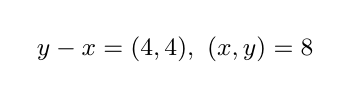
\begin{tikzpicture}
    \begin{scope}[xshift=-4.0cm,scale=.34]
      \HexPatch{-2/0,-1/0,0/0,1/0,2/0,3/0,
        0/-2,0/-1,0/1,0/2,0/3,
        -2/2,-1/1,1/-1,2/-2,3/-3}
      \HexWindow[fill=black!7,draw=none]{-2}{0}{1}{0}
      \HexWindow[fill=black!11,draw=none]{0}{-2}{0}{1}
      \HexWindow[fill=black!15,draw=none]{-2}{2}{1}{-1}
      \HexAttacker{0}{0}
    \end{scope}
    \begin{scope}[xshift=4.0cm,scale=.34]
      \HexPatch{-2/0,-1/0,0/0,1/0,2/0,3/0,
        0/-2,0/-1,0/1,0/2,0/3,
        -2/2,-1/1,1/-1,2/-2,3/-3}
      \HexWindow[fill=black!7,draw=none]{-2}{0}{1}{0}
      \HexWindow[fill=black!11,draw=none]{0}{-2}{0}{1}
      \HexWindow[fill=black!15,draw=none]{-2}{2}{1}{-1}
      \HexAttacker{0}{0}
    \end{scope}
    \draw[<->,densely dashed] (-1.7,0) -- node[fill=white,font=\small]
      {$y-x=(4,4),\ \dist(x,y)=8$} (1.7,0);
  \end{tikzpicture}
  \caption{Counterexample 1, schematically.  The two attacker placements are
  at hex distance $8$, off all three axes, and have disjoint clean window
  stars.  Together they enroll 36
  one-stone windows, and the potential jumps from $0$ to
  $36\lambda^{-5}=4/\sqrt3>1$.  Three of the 18 windows through each new
  stone are shaded.}
  \label{fig:es-birth}
\end{figure}

\subsection{Practical domain and open boundary}

The exact node test can be performed without floating-point arithmetic.

\begin{corollary}[Integer-only threshold check; companion Corollary 2]
\label{cor:ES-C2}
At a nonterminal position, for $s=1,\ldots,5$, let $n_s$ be the number of
currently attacker-alive windows with exactly $s$ attacker stones.  Put
\[
  a=n_1+3n_3+9n_5,
  \qquad b=n_2+3n_4.
\]
Then
\[
  \Phi<1
  \quad\Longleftrightarrow\quad
  b\le8,\qquad a^2<3(9-b)^2.
\]
\end{corollary}

Indeed, $\Phi<1$ is $a+\sqrt3b<9\sqrt3$.  The right side of
$a<\sqrt3(9-b)$ must be positive, giving $b\le8$, after which squaring is
equivalent.  This check costs $O(\#\text{touched windows})$, not
$O(\#\text{threats})$.

If $I=\sum_{s=1}^5s n_s$ is the number of attacker-stone/alive-window
incidences, then $\Phi\ge I/18$.  Thus $\Phi<1$ forces $I\le17$.  With $N_A$
attacker stones, all but at most 17 of the $18N_A$ incidences must already lie
in defender-killed windows.  The practical domain is therefore a heavily
blocked, endgame-like region rather than a general middlegame.

The raw global claim that $\Phi<1$ blocks the unrestricted infinite game
forever remains open.  Counterexample 1 starts with $\Phi=0$ and, after the
fixed zero-danger fillers, uses two far placements to birth 36 one-stone
windows, producing $4/\sqrt3>1$ as shown in \cref{fig:es-birth}.  Requiring
that no current attacker window have at most two empties does not repair the
invariant, because the condition holds vacuously at $\Phi=0$ before the same
births.  Replacing $\Phi<1$ by $\Phi\le1$ also fails: three separated count-$4$
targets have total potential $1$, the defender kills at most two, and the
attacker completes the survivor.  These are failures of the proposed
potential certificates, not proofs that the attacker wins every corresponding
unrestricted game.  The $\Phi=1$ example is a static blanket-game
construction; it is not asserted to be a material-balanced reachable engine
position and does not prove sharpness after restriction to reachable nodes.

Every positive-reduction greedy placement lies in an attacker-touched alive
window and therefore inside the relevance closure of \cref{sec:computable-zones}.
If no monitored window remains, one or both placements of a defender turn may
instead be arbitrary legal fillers.  The certified strategy must permit these
fillers.  Their presence does not affect the dismissal soundness theorem; it
only constrains the potential-certified strategy.

\section{Domination patterns}
\label{sec:domination}

Domination compares a searched defender reply with an omitted reply over a
finite stopped horizon.  The comparison transfers complete strategies and
checks occupancy, window masks, and the legality frontier after every mapped
placement.  This prevents local mask similarity from hiding a different legal
continuation.

For a cell $x$, write $B_R(x)=\{z:\dist(x,z)\le R\}$ and let $\Omega(x)$ be
the 18 windows containing $x$.  For a post-opening position $P$, define its
geometric support by
\[
  \Lambda(P)=\bigcup_{s\in\Stones(P)}B_8(s).
\]
If $P$ is nonterminal, its legal placements are
$L(P)=\Lambda(P)\setminus\Stones(P)$; if $P$ is terminal, $L(P)=\varnothing$.
An empty cell is \emph{dead} when every window in $\Omega(x)$ is dead.

\subsection{Stopped outcomes and causal simulation}

The outcome records the first terminal placement, with the defender's reply
itself at time zero.

\begin{definition}[Stopped horizon outcome; companion D3 and D4]
\label{def:Dom-D3}
Let $S$ be a possibly terminal successor of a defender reply.  A horizon $n$
allows at most $n$ further placements after that reply.  Given pure
continuation strategies $\sigma_D$ and $\tau_A$, play stops at the first
terminal placement or after those $n$ placements, and
\[
  \operatorname{Out}_n(S,\sigma_D,\tau_A)
  \in\{D@t:0\le t\le n\}\cup
      \{A@t:0\le t\le n\}\cup\{?\}.
\]
Here $? $ means that no terminal placement occurred through the horizon.  For
defender comparison, set
\[
  u_D(D@t)=1,
  \qquad u_D(?)=0,
  \qquad u_D(A@t)=-1.
\]
Winning windows and times remain in the trace, although all wins by one player
have the same qualitative value.  A pure $X$-strategy assigns a legal
placement to every nonterminal history of length less than $n$ at which $X$
is to place, including both consecutive histories of an $X$ turn, and is
never queried after a terminal history.  Write $\Sigma_X(S)$ for the set of
such strategies from $S$.
\end{definition}

The transfer directions encode the defender-pruning implication.

\begin{definition}[$n$-outcome domination; companion D5 and Lemma 3]
\label{def:Dom-D5}
Let $a$ and $b$ be legal defender replies at the same nonterminal position
$P$, with stopped successors $S_a=P+a$ and $S_b=P+b$.  The reply $b$ is
\emph{$n$-outcome-dominated by $a$ for the defender}, written
$b\preceq_n a$, if there are maps
\[
  T_D:\Sigma_D(S_b)\to\Sigma_D(S_a),
  \qquad
  T_A:\Sigma_D(S_b)\times\Sigma_A(S_a)\to\Sigma_A(S_b)
\]
such that, for every discarded-branch defender strategy $\sigma_b$ and every
searched-branch attacker strategy $\tau_a$,
\[
 u_D\!\left(\operatorname{Out}_n
     (S_a,T_D(\sigma_b),\tau_a)\right)
 \ge
 u_D\!\left(\operatorname{Out}_n
     (S_b,\sigma_b,T_A(\sigma_b,\tau_a))\right).
\]
Equivalently,
\[
  \forall\sigma_b\ \exists\sigma_a\
  \forall\tau_a\ \exists\tau_b:\quad
  u_D(\operatorname{Out}_n(S_a,\sigma_a,\tau_a))
  \ge u_D(\operatorname{Out}_n(S_b,\sigma_b,\tau_b)).
\]
Consequently, an attacker win forced by the horizon after the searched reply
$a$ is also forced after the omitted reply $b$.
\end{definition}

A causal simulation is the checkable witness used by the patterns below.

\begin{definition}[Causal alternating simulation; companion D6]
\label{def:Dom-D6}
A depth-$k$ defender-favouring alternating simulation relates a searched state
$G$ to an omitted state $H$ at equal placement depth.  A defender-terminal
$G$, or an attacker-terminal $H$, is accepted immediately.  An
attacker-terminal $G$ is accepted only if $H$ is already attacker-terminal;
a defender-terminal $H$ is accepted only if $G$ is already
defender-terminal.  No move is generated after a terminal state.  Two
nonterminal states are accepted when $k=0$.

Otherwise the states have the same player to move and the same remaining
placement budget.  At a defender history, every legal move in $H$ is mapped
causally to a legal move in $G$.  At an attacker history, every legal move in
$G$ is mapped causally to a legal move in $H$.  The successor pair is related
at depth $k-1$.  The map depends only on the paired prefix and current move.
It pairs \textup{FirstStone} with \textup{FirstStone} and
\textup{SecondStone} with \textup{SecondStone}, including stored first-cell
coordinates under any coordinate involution.
\end{definition}

Such a simulation implies $n$-outcome domination by recursively transferring
the two players' strategies \cite{hexobot-companions}.  Each simulation step
must account for three channels: the mapped cells must be empty with explicit
images for branch-exclusive empties; after each mapped placement, every
labelled mask in the union of the two incident 18-window sets must be compared,
with the terminal clauses applied before phase advance; and legal moves must
be included in the actor-dependent direction.

\subsection{Dead cells and interchangeable hits}

A dead empty has no legality frontier because the dead-window witnesses on
the six directed rays already support its whole radius-eight ball.

\begin{lemma}[A dead empty has no legality frontier; companion Lemma 7]
\label{lem:Dom-L7}
Let $b$ be empty and dead in a nonterminal post-opening position $P$.  Then
\[
  B_8(b)\subseteq\Lambda(P).
\]
In particular, $b$ is legal, and placing at $b$ inserts no previously
unsupported cell into the legal store.
\end{lemma}

\begin{proof}
Let $u$ range over the six directed axial unit vectors.  The endpoint window
\[
  W_u=\{b,b+u,\ldots,b+5u\}
\]
belongs to $\Omega(b)$.  It is dead while $b$ is empty, so among
$b+u,\ldots,b+5u$ there is an old stone
$s_u=b+k_u u$ with $1\le k_u\le5$.

Take $z\in B_8(b)$.  It lies in a closed $60^\circ$ sector between adjacent
directed axes $u$ and $v$, so
\[
  z-b=\alpha u+\beta v,
  \qquad \alpha,\beta\ge0,
  \qquad \alpha+\beta=\dist(b,z)\le8.
\]
After a rotation or reflection, take $u=(1,0)$ and $v=(0,1)$, and write
$s=s_u=b+ku$ with $1\le k\le5$.  Then
\[
  \dist(z,s)=
  \max\{|\alpha-k|,\beta,|\alpha+\beta-k|\}\le8,
\]
because $\alpha$, $\beta$, $\alpha+\beta$, and $k$ all lie in $[0,8]$.
Thus $z\in B_8(s)\subseteq\Lambda(P)$.  This holds for every $z$.
\end{proof}

Deadness makes the omitted reply frontier-inert, but it does not impose the
same condition on the searched substitute.

\begin{proposition}[Frontier-certified dead-cell dismissal; companion P1]
\label{prop:Dom-P1}
Let $P$ be a nonterminal post-opening position with the defender to place.
Let $a\ne b$ be legal empty cells.  Assume every window in $\Omega(b)$ is
already dead in $P$.  Unless $P+a$ is an immediate defender win, also assume
\[
  \Lambda(P)\cup B_8(a)=\Lambda(P)\cup B_8(b).
\]
Then $b\preceq_n a$ for every finite $n$.  By \cref{lem:Dom-L7}, the displayed
condition is equivalent here to $B_8(a)\subseteq\Lambda(P)$.  Thus $b$ may be
dismissed in favor of any searched $a$ that either wins immediately or is
frontier-inert.  Deadness of $b$ does not make this separate obligation on
$a$ automatic.
\end{proposition}

\begin{proof}[Proof idea; complete proof in the companion]
Compare $P+a$ and $P+b$ by transposing $a$ and $b$ until the counterpart is
used.  The hypotheses synchronize legal support.  Every window through $b$
is permanently dead, while the remaining changed windows either agree or
change ownership in the defender-favouring direction.  The occupancy,
terminality, and frontier channels therefore give an all-depth causal
simulation; an immediate defender win after $a$ is already maximal.  See
\cite{hexobot-companions}.
\end{proof}

Two hits of one count-$4$ threat become symmetric only after every other
incident window is made inert and the successor supports agree.

\begin{proposition}[Dead-spoke interchangeable hits; companion P2]
\label{prop:Dom-P2}
Let $P$ be a nonterminal post-opening position with the defender to place.
Let $W$ be an attacker-alive window with exactly four attacker stones and
exactly two empty cells $x\ne y$.  Both $x$ and $y$ are legal.  Assume
\[
  (\Omega(x)\cup\Omega(y))\setminus\{W\}
\]
consists entirely of windows already dead in $P$, and assume
\[
  \Lambda(P)\cup B_8(x)=\Lambda(P)\cup B_8(y).
\]
Then the replies are mutually outcome-dominating at every horizon:
\[
  x\preceq_n y,
  \qquad
  y\preceq_n x
  \qquad(n<\infty).
\]
A solver may retain one canonical member of $\{x,y\}$ at that defender node.
\end{proposition}

\begin{proof}[Proof idea; complete proof in the companion]
Either defender hit kills $W$.  The dead-spoke premise then makes every window
through either special cell permanently dead.  Transposing $x$ and $y$
preserves occupancy choices, the support equality preserves legal moves in
both directions, and every mask outside the dead union is identical.  This is
an outcome-preserving bisimulation at all depths.  See
\cite{hexobot-companions}.
\end{proof}

Equality of count profiles is insufficient.  Labelled empty cells and the
window-intersection hypergraph can change minimum hitting sets or
fork-creating cells even when every pair $(\cnt_A,\cnt_D)$ agrees.  A broader
equivalence would have to preserve labelled masks, incidence, occupancy, and
radius-eight support throughout the $n$-causal cone.  The dead-spoke premise
avoids that unproved classification.

\begin{figure}[tbp]
  \centering
  \begin{tikzpicture}[scale=.52]
    \HexPatch{-1/0,0/0,1/0,2/0,3/0,4/0,5/0,6/0,
      2/-1,2/1,1/1,3/-1,4/-1,4/1,3/1,5/-1}
    \HexWindow[window one]{0}{0}{1}{0}
    \draw[black!45,line width=2.2pt]
      \HexAt{2}{-1} -- \HexAt{2}{0} -- \HexAt{2}{1};
    \draw[black!45,line width=2.2pt]
      \HexAt{1}{1} -- \HexAt{2}{0} -- \HexAt{3}{-1};
    \draw[black!45,line width=2.2pt]
      \HexAt{4}{-1} -- \HexAt{4}{0} -- \HexAt{4}{1};
    \draw[black!45,line width=2.2pt]
      \HexAt{3}{1} -- \HexAt{4}{0} -- \HexAt{5}{-1};
    \HexAttacker{0}{0}\HexAttacker{1}{0}
    \HexAttacker{3}{0}\HexAttacker{5}{0}
    \HexMark{2}{0}{dot}{}\HexMark{4}{0}{dot}{}
    \HexAttacker{2}{-1}\HexDefender{2}{1}
    \HexAttacker{1}{1}\HexDefender{3}{-1}
    \HexDefender{-1}{0}
    \HexAttacker{4}{-1}\HexDefender{4}{1}
    \HexAttacker{3}{1}\HexDefender{5}{-1}
    \HexDefender{6}{0}
  \end{tikzpicture}
  \caption{A representative dead-spoke configuration.  The highlighted
  threat has four attacker stones and the two marked empty hits.  Three spoke
  directions per hit show old attacker and defender witnesses.  The P2
  premise applies this deadness condition to all 17 other windows through
  each marked cell, not only the representative spokes shown.}
  \label{fig:dead-spoke}
\end{figure}

\subsection{Same-turn commutation}

Two placements may be sorted only when both were legal before the turn and
neither possible first placement wins.

\begin{proposition}[Nonwinning-prefix turn commutation; companion P3]
\label{prop:Dom-P3}
Let $P$ be a nonterminal \textup{FirstStone} position for either player $X$.
Let $p\ne q$ be legal already in $P$, and suppose neither $P+p$ nor $P+q$ is
terminal.  Then both traces $p;q$ and $q;p$ are legal and have the same
qualitative rule outcome after the second placement.  If nonterminal, they
have identical occupancy, labelled window masks, legal support, player to
move, and \textup{FirstStone} phase.  If terminal, both terminate on the
second placement with winner $X$ and the same absolute placement count.
\end{proposition}

\begin{proof}[Proof idea; complete proof in the companion]
Initial legality makes either second cell remain legal, and the final support
$\Lambda(P)\cup B_8(p)\cup B_8(q)$ is order-independent.  Inserting the two
owner bits into every window mask commutes, including in a window containing
both cells.  The singleton-nonterminal premises exclude a first-placement
win; any joint win is therefore completed by the second placement in both
orders.  See \cite{hexobot-companions}.
\end{proof}

The live engine states need not be field-identical.  Ordered history,
last-turn metadata, serialized order, and the retained terminal
\textup{SecondStone} first-cell payload may differ.  The proposition equates
rule outcomes, not these order-sensitive features or the two intermediate
\textup{SecondStone} threat states.

\begin{figure}[tbp]
  \centering
  \begin{tikzpicture}[
      position node/.style={draw,rounded corners=2pt,minimum width=2.4cm,
        minimum height=.8cm,fill=black!3},
      every edge/.style={draw,-{Stealth[length=5pt]}}]
    \node[position node] (P) {$P$};
    \node[position node,right=3.2cm of P] (Pp) {$P+p$};
    \node[position node,below=1.7cm of P] (Pq) {$P+q$};
    \node[position node,right=3.2cm of Pq] (Ppq) {$P+\{p,q\}$};
    \path (P) edge node[above] {$p$} (Pp)
              edge node[left] {$q$} (Pq)
          (Pp) edge node[right] {$q$} (Ppq)
          (Pq) edge node[below] {$p$} (Ppq);
  \end{tikzpicture}
  \caption{The commuting square for two same-turn placements.  Both paths
  reach the same completed-turn rule state under the premises of P3.}
  \label{fig:commutation}
\end{figure}

The analytic proofs have randomized local checks, not exhaustive machine
proofs.  MV-P3 tested 2,997 random legal same-mover pairs under the
singleton-nonwin filter and found 0 commutation mismatches.  MV-L7 tested 400
adversarial dead-cell configurations and found 0 legality-frontier violations;
the worst minimum distance from a cell of the radius-eight ball to an old
stone was $6$, leaving margin $2$.  Full exhaustive quotient enumeration
remains open.

These results do not claim that an arbitrary frontier-extending reply can
substitute for a dead cell, that equal window counts make hitting cells
interchangeable, or that stones of one colour are globally monotone-helpful
when legal frontiers differ; no transferred strategy continues after a
terminal placement, and the prospective exhaustive enumerations are
specifications rather than executed evidence.

\section{Mechanized validation}
\label{sec:validation}

The validation harness uses a mini-model solver that was checked
move-for-move against the \emph{hexo\_engine} implementation.  These runs
tested the predecessor closure as a search generator.

Two closure experiments were executed.  First, the closure-restricted solver
did not claim the engineered junction position.  The junction cell was in the
closure, and the defender survived after 1,396 uncapped nodes.  Second, a
bounded random check covered 91 attackable positions.  The closure-restricted
solver made 52 \textsc{win} claims, with no divergence from the full legal
move set at the matched horizon; the run took 139 seconds.  As a negative
control, the earlier radius-2 experiments used the same harness and produced
false \textsc{win} claims for unsound restrictions.

These experiments are search-behavior evidence for the predecessor heuristic.
They do not validate the revised ranked closure in \cref{thm:T7} and are not
part of the proofs of \cref{thm:T3,thm:T4,thm:T7}.  The separate
machine-verification status of the domination patterns is summarized in
\cref{sec:domination}.

\section{Open problems}
\label{sec:open-problems}

\paragraph{Sharpened budget.}
The local budget $B$ and exposure $E^\D$ still count every defender placement
before the relevant local resolution or exposure stop.  A sharper debit would
combine quiet placements $F$ with a per-window forced-hit capacity $H_W$.
This requires branchwise worst-case bookkeeping.  No theorem here proves that
compulsory hits are unavailable for filling a selected window, so the problem
remains open.

\paragraph{Resolved frontier accounting.}
The role radius $8(r-1)$, uniformly $8(B-1)$, and the touched--virgin split
resolve the earlier band-accounting problem.  The virgin radius
$8(E^\D-6)$ is sharp at exposure $7$.

\paragraph{Pairing at the threshold.}
The density bound in \cref{cor:T8.1} leaves $k=7$ and $g=3$ open, where the
required matched density is exactly one.  This threshold case does not affect
Hexo, whose winning length is $k=6$.  Existence at the threshold remains
unsettled.

\paragraph{Formalization.}
The model and results through \cref{thm:T10} are finite combinatorics and are
feasible to formalize in Lean or Coq.  Such a formalization would provide a
reference checker for \cref{zone:Z2,zone:Z4},
\hyperref[zone:Z5prime]{clause \textup{(Z5$'$)}}, the $B$, $E^\D$, and $r$
inequalities, transition-inclusive envelopes, and DAG label and clock
consistency.

\appendix
\clearpage
\section{Notation reference}
\label{sec:notation}

\begin{table}[!htbp]
  \centering
  \caption{Notation used in the main text.}
  \label{tab:notation}
  \renewcommand{\arraystretch}{1.08}
  \begin{tabular}{@{}p{.22\textwidth}p{.50\textwidth}p{.20\textwidth}@{}}
    \toprule
    Symbol & Meaning & Defining location \\
    \midrule
    $d(x,y)$ & Hex distance between cells $x$ and $y$. & \cref{def:D1} \\
    $\mathfrak a$ & An axis vector in $\{(1,0),(0,1),(1,-1)\}$. & \cref{def:D2} \\
    $W$ & A six-cell window along one axis. & \cref{def:D2} \\
    $\cnt_X(W,P)$ & Number of stones of player $X$ in $W$ at $P$. & \cref{def:D3} \\
    alive, dead, threat & Window states determined by the two colour counts. & \cref{def:D5} \\
    $\ownwinnow(P)$ & Current-turn completion predicate for the mover. & \cref{def:D6} \\
    $\hit(P)$ & Multiset of empty-cell sets of opponent threat windows. & \cref{def:D6} \\
    $\mhs(P)$ & Minimum size of a set meeting every member of $\hit(P)$. & \cref{def:D6} \\
    ply & One placement, indexed absolutely along a play. & \cref{def:D7} \\
    $\mathfrak D(P,T)$ & Defender placements strictly before horizon ply $T$. & \cref{def:D7} \\
    $\operatorname{core}(\mathcal C,N)$ & Certificate cells and witness windows below node $N$. & \cref{def:D10} \\
    $\Prot(N)$ & Core together with defender completion-guard empties. & \cref{def:D11} \\
    $S(N)$ & Searched legal defender replies at AND node $N$. & \cref{def:D9} \\
    $\Legal(P)$ & Legal empty placement cells in position $P$. & \cref{def:D4} \\
    $\Stones(P)$ & Occupied cells in position $P$. & \cref{def:D3} \\
    $B_r(U)$ & Cells within distance $r$ of some cell of $U$; written $B(r;U)$ in the main theorem. & \cref{def:D11} \\
    $\operatorname{hitting}(P)$ & Union of the empty sets of attacker-threat windows. & \cref{thm:T4} \\
    $R(P,D)$ & Horizon relevance-closure candidate generator. & \cref{def:D13} \\
    $X$ & Real-only dismissed defender stones in the coupling. & \cref{def:D12} \\
    $Y$ & Ghost-only searched filler defender stones in the coupling. & \cref{def:D12} \\
    $\widehat X$ & History of every cell ever added to $X$. & \cref{def:D12} \\
    $\Phi(P)$ & Dynamic potential of attacker-touched alive windows. & \cref{def:ES-D3} \\
    $\lambda$ & Potential base $\sqrt3$. & \cref{def:ES-D3} \\
    $\Psi_F(P)$ & Residual potential for a fixed target family $F$. & \cref{def:ES-D3} \\
    \bottomrule
  \end{tabular}
\end{table}

\begin{table}[p]
  \centering
  \caption{Crosswalk from paper numbering to source tags in the repository
  proof document.}
  \label{tab:source-crosswalk}
  \renewcommand{\arraystretch}{.98}
  \begin{tabular}{@{}p{.24\textwidth}p{.15\textwidth}p{.51\textwidth}@{}}
    \toprule
    \multicolumn{1}{l}{Paper number} &
    \multicolumn{1}{l}{Source tag} & \multicolumn{1}{l}{Name} \\
    \midrule
    \Cref{def:D1} & D1 & Board, cells, and distance \\
    \Cref{def:D2} & D2 & Axes and windows \\
    \Cref{def:D3} & D3 & Positions \\
    \Cref{def:D4} & D4 & Legality and transitions \\
    \Cref{def:D5} & D5 & Window states \\
    \Cref{def:D6} & D6 & $\lambda^1$ predicates \\
    \Cref{def:D7} & D7 & Plies and horizon \\
    \Cref{def:D8} & D8 & Dominance direction \\
    \Cref{def:D9} & D9 & Certificate grammar \\
    \Cref{def:D10} & D10 & Certificate core \\
    \Cref{def:D11} & D11 & Zone-carrying certificate \\
    \Cref{def:D12} & D12 & Real--ghost coupling \\
    \Cref{def:D13} & D13 & Horizon relevance closure \\
    \Cref{fact:F1} & F1 & Window collinearity \\
    \Cref{lem:L1} & L1 & Packing bound \\
    \Cref{lem:L2} & L2 & Boundary pair \\
    \Cref{lem:L3} & L3 & Difference accounting \\
    \Cref{lem:L4} & L4 & Permanence \\
    \Cref{lem:L5} & L5 & Inert-extension transfer \\
    \Cref{lem:L6} & L6 & Deletion monotonicity and well-formed legality \\
    \Cref{lem:L7} & L7 & Completion counting \\
    \Cref{prop:prot-mono} & (unnumbered) & Monotonicity of protection \\
    \Cref{lem:L9} & L9 & Frontier chain closure \\
    \Cref{lem:L10} & L10 & Short-range attacker-core containment \\
    \Cref{thm:T1} & T1 & Single-turn tactical locality \\
    \Cref{thm:T2} & T2 & Threat-creation locality \\
    \Cref{thm:T3} & T3 & Horizon-parameterized dismissal soundness \\
    \Cref{thm:T4} & T4 & Zone reading \\
    \Cref{thm:T5} & T5 & Static-set coverage for short horizons \\
    \Cref{thm:T6} & T6 & Forced-tree regime \\
    \Cref{thm:T7} & T7 & Closure and certificate-extras coverage \\
    \Cref{thm:T8} & T8 & No pairing \\
    \Cref{cor:T8.1} & T8.1 & Translation-invariant line grids \\
    \Cref{zone:Z1} & Z1 & Hitting condition \\
    \Cref{zone:Z2} & Z2 & Protection condition \\
    \Cref{zone:Z4} & Z4 & Well-formed attacker legality \\
    \Cref{zone:Z5} & Z5 & Horizon-scaled frontier guard \\
    \Cref{eq:MI} & MI & Anchored defender-count inequality \\
    \bottomrule
  \end{tabular}
\end{table}

\clearpage


\section*{Acknowledgments}
The underlying proof documents were drafted and adversarially reviewed with the assistance of AI systems (Claude and GPT-family models) and machine-checked where stated.

\bibliographystyle{hexopaper}
\bibliography{refs}

\end{document}
